\documentclass[12pt, twoside]{book}

% Language settings
\usepackage[catalan]{babel}

% Page settings
\usepackage[a4paper,width=150mm,top=25mm,bottom=25mm]{geometry}

% Headers and 
\usepackage{fancyhdr}

% Picture captions
\usepackage[font=small,labelfont=bf]{caption}

% No sé què fa acò, averiguar
%\usepackage{microtype}

% Encoding
\usepackage[utf8]{inputenc}
\usepackage[T1]{fontenc}

% Mathematical notation
\usepackage{mathtools}
\usepackage{amssymb}

% Not sure
%\usepackage{txfonts}

% Graphics
\usepackage{graphicx}
\graphicspath{{images/}}

\usepackage{wrapfig}

% Settings
%\pagestyle{plain}

% Better references
\usepackage{cleveref}% load last
\crefname{equation}{}{}
\Crefname{equation}{}{}
\crefname{figure}{}{}
\Crefname{figure}{}{}
\newcommand{\crefrangeconjunction}{-}
\newcommand{\crefpairconjunction}{-}
\newcommand{\crefmiddleconjunction}{-}
\newcommand{\creflastconjunction}{-}


% Customized commands

% Positioning
\newcommand*{\sub}[1]{_{\text{\tiny #1}}}
\newcommand*{\abs}[1]{\left\rvert #1 \right\lvert}
\newcommand*{\pd}[3][]{\frac{\partial ^{#1} #2}{\partial #3 ^{#1}}}

\newcommand*{\rfun}{( \vec r)}
\newcommand*{\rtfun}{(\vec r, t)}

% Symbols 
\newcommand*{\Zahl}{\mathbb Z} % Integers 
\newcommand*{\Nat}{\mathbb N} % Naturals
\newcommand*{\Real}{\mathbb R} % Reals
\newcommand*{\Comp}{\mathbb C} % Complex

\renewcommand{\jmath}{j}

\renewcommand*{\Re}{\operatorname {Re}}
\renewcommand*{\Im}{\operatorname {Im}}

\newcommand*{\e}[1]{\operatorname{e}^{#1}} % actualitzar en caps 1 i 2
\newcommand*{\del}{\vec \nabla}
\newcommand*{\curl}{\del \times} 

  % Doc specific
\renewcommand*{\l}{\ell}

\newcommand*{\ux}{\hat u_x}
\newcommand*{\uy}{\hat u_y}
\newcommand*{\uz}{\hat u_z}
\newcommand*{\us}{\hat u_s}
\newcommand*{\uf}{\hat u_{\varphi}}

\newcommand*{\vp}{V_0 ^+}
\newcommand*{\vm}{V_0 ^-}
\newcommand*{\ip}{I_0 ^+}
\newcommand*{\im}{I_0 ^-}

\newcommand*{\Bf}{\mathcal J}
\newcommand*{\Bs}{\mathcal N}

\newcommand*{\rfield}[1]{\vec{\mathcal{#1}}}

\title{
Ones electromagnètiques\\
Universitat de València\\
Curs 2015-2016\\
}

\author{\small{\texttt{llacan@alumni.uv.es}}}
\date{}
%%%%%%%%%%%%%%%%%%%%%%%%%%%%%%%%%%%%%%%%%%%%%%%%%%%%%%%%%%%%%%%%%%

\begin{document}

\maketitle

\tableofcontents

\mainmatter

\chapter{Sistemes guiats amb simetria translacional}

\section{Introducció}

Una guia d' ona és una estructura que restringeix l' expansió d' una ona a una regió de l' espai, de manera que aquesta és propaga desde la font fins a un lloc desitjat minimitzant la pèrdua d' energia. En general consisteixen en una capa de material conductor que envolta la regió de propagació, com a la figura \cref{fig:waveguide}.

\begin{figure}[ht]
  \centering
  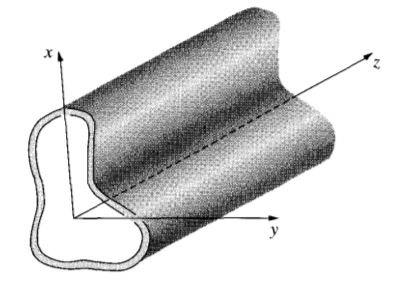
\includegraphics[scale=0.4]{arbitrary}
  \caption{Guia d' ona amb simetria translacional}
  \label{fig:waveguide}
\end{figure}

\section{Ones electromagnètiques}

Per a estudiar el comportament del camp electromagnètic en presència de conductors necessitem resoldre les equacions de Maxwell en zones sense càrrega (i.e. $\rho = \vec J = 0 $) junt a les condicions de contorn imposades pel sistema. 

\begin{subequations}
  \begin{align}
     \del \rfield D &= 0, \label{ME1}\\
     \curl \rfield E &= - \pd{\rfield B}{t}, \label{ME2}\\
     \del \rfield B &=0,  \label{ME3}\\
     \curl \rfield H &= \pd{\rfield D}{t} \label{ME4}
  \end{align}
\end{subequations}

Açò es simplifica als sistemes amb simetria translacional, en que les propietats dels material són constants al llarg d' una direcció espacial. Com que les propietats dels materials seran constants suposarem també que el perfil temporal del camp, que depén sobretot de la font, es manté amb el temps, i que aquest perfil és harmònic amb el temps, de manera que podem separar els camps en dos components (en general treballarem amb camps imaginaris, entenent que en realitat el camp és sols la part real):

\begin{subequations}
  \begin{align}
    \rfield E \rtfun = E\rfun\e{\jmath \omega t} \label{harmE}\\
    \rfield H \rtfun = H\rfun\e{\jmath \omega t} \label{harmH}
  \end{align}
\end{subequations}

Aquesta suposició simplifica enormement les matemàtiques, i en casos en que la font no és harmònica  podem utilitzar anàlisi de Fourier i descomposar-la en components que si ho són. La majoria de les fonts, de qualsevol manera, són d' aquest tipus.

Si substituim \cref{harmE,,harmH} en \cref{ME1,ME2,ME3,ME4} obtenim equacions de Helmholtz \footnote{Sempre i quan el medi siga lineal, isòtop i homogeni, cosa que suposarem durant tot el curs. També donarem per sentat que el medi no és magnètic, pel que $\mu{}_r  \sim 1$.}:

\begin{subequations}
    \label{helm}
  \begin{align}
    \del ^2 \vec E + k^2 \vec E &= 0 \\
    \del ^2 \vec H + k^2 \vec H &= 0 
  \end{align}
\end{subequations}

on $k = \omega \sqrt{\epsilon \mu} \nonumber$. Tenim ara sis equacions per a les components dels camps que podem resoldre per separació de variables. Resoldrem sols el cas $E_x$, ja que la resta són anàlegs:

\begin{equation}
  \label{eqdiffex}
  \pd[2]{E_x}{2} + \pd[2]{E_x}{t} + \pd[2]{E_x}{t} + k^2 E_x = 0
\end{equation}

Suposem $E_x \rfun = e_1(x)e_2(y)e_3(z)$, i com que $z$ és privilegiada (el material és simètric en aquesta direcció), fem $ E_x \rfun = f_t(x, y) f_z(z)$. Pel procediment habitual convertim \cref{eqdiffex} en dues noves:

\begin{equation}
  \frac{1}{f_z}\pd[2]{f_z}{t} = - \beta ^2
\end{equation}

\begin{equation}
  \frac{1}{f_t} \left(\pd[2]{f_t}{x} + \pd[2]{f_t}{y} \right ) + k^2 = \beta ^2
\end{equation}

On $\beta$ és un paràmetre independent que desconeixem. El signe i el quadrat han sigut introduïts per conveniència.

La solució de la primera és $f_z(z) \propto \e{ \pm \jmath \omega t}$. La segona és un altra equació de Helmholtz que deixem sense resoldre:

\begin{equation}
  \pd[2]{f_t}{x} + \pd[2]{f_t}{y}  + (k^2 - \beta ^2) f_t = 0
\end{equation}

Fent el mateix amb les altres 5 equacions obtenim camps harmònics en $z$ amb freqüència espacial $\beta$:

\begin{align}
  \rfield E \rtfun = ( \vec{e_t} + \vec e_z ) \e{\jmath(\omega t - \beta z)}  \\
  \rfield H \rtfun = ( \vec{h_t} + \vec h_z ) \e{\jmath(\omega t - \beta z)}
\end{align}

En principi tenim sis equacions, però podem reduir-les a dues si utilitzem les equacions de Maxwell sobre els camps. Usarem l' operador $\del$ descompost:

\begin{equation}
  \del = \pd{\,}{x}\ux + \pd{\,}{y}\uy +\pd{\,}{z}\uz = \del _t - \jmath \beta \vec u_z
\end{equation}

La component $z$ és queda així perquè anem a aplicar l' operador sobre camps harmònics en $z$, pel que $\pd{}{z}$ té el mateix efecte que multiplicar per $-\jmath \beta$.

Aplicant la llei de Faraday \cref{ME2} a aquests camps obtenim

\begin{equation}
  (\del_t-\jmath\beta\uz)\times (\vec e_t +\vec e_z) = -\jmath\omega\mu (\vec h _t + \vec h_z) 
\end{equation}

Separant els resultats en components $z$ i $T$:

\begin{equation}
  \del _t \times \vec e_t = -\jmath \omega\mu(\vec h_z ) \label{eT}
\end{equation}

\begin{equation}
  -\uz \times (\del _t \vec e_z ) -\jmath \omega \times \vec e_t = -\jmath \omega \mu \vec h _t \label{eZ}
\end{equation}

Fent el mateix amb la llei d' Ampère \cref{ME4} s' obté:

\begin{equation}
  \del _t \times \vec h_t = \jmath \omega\epsilon(\vec e_z) \label{hT}
\end{equation}

\begin{equation}
  -\uz \times (\del _t \vec h_z ) -\jmath \omega \times \vec h_t = -\jmath \omega \epsilon \vec e _t \label{hZ}
\end{equation}

Si $e_z = h_z = 0$ tenim que $\del_t \times e_t = \del_t \times h_t = 0$ existeixen potencials escalars i vectorials i el problema és redueix a resoldre les equacions de Laplace per a aquests. En cas contrari podem aïllar $\vec h_t $ en \cref{eZ} i $\vec e_t$ en \cref{hZ} i substituir en \cref{eT} i \cref{hT}, per obtindre les expressions:

\begin{equation}
  \label{soleT}
  \vec e_t = \frac{\jmath}{\beta ^2 - \omega ^2 \mu\epsilon} (\beta \del _t \vec e_z + \omega \mu \del _t \times \vec h_z )
\end{equation}

\begin{equation}
  \label{solhT}
  \vec h_t = \frac{\jmath}{\beta ^2 - \omega ^2 \mu\epsilon} (\beta \del _t \vec h_z - \omega \epsilon \del _t \times \vec e_z )
\end{equation}

Si usem aquestes expressions en \cref{eT} i \cref{hT} junt a l' identitat $\del \times (\curl \vec A ) = \del (\del \cdot \vec A) - \del ^2 \vec A$ i \cref{ME1,ME3} arribem a dues equacions de Helmholtz per als components en $z$:

\begin{equation}
  \label{helmhz}
  \del ^2 h_z + (k^2 - \beta ^2) h_z = 0
\end{equation}

\begin{equation}
  \label{helmez}
  \del ^2 e_z - (k^2 - \beta ^2) e_z = 0
\end{equation}

Per a calcular $\rfield E$ i $\rfield H$ en tot l' espai, per tant, hem de resoldre aquestes equacions junt a les condicions de contorn apropiades i obtindre $e_z$, $h_z$ i $\beta$, dels quals podem obtindre $\vec e_t$ i $\vec h_t$.

\section{Espectre mode i propietats de tall}

\subsection{Modes TEM}

Si $e_Z = h_Z = 0 $ les solucions per als camps s' anomenen modes TEM (transversal electromagnètic) i són particularment simples. De \cref{eT,hT} tenim que $\del_t \times \vec e_t = \del_t \times \vec h_t = 0$, i com hem dit abans podem utilitzar mètodes d' electrostàtica per a obtindre els components transversals. De \cref{eZ,hZ} tenim que

\begin{figure}[ht]
  \centering
  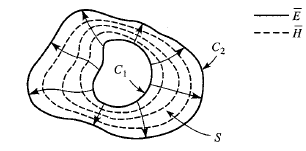
\includegraphics[scale=0.5]{arbitraryTEM}
  \caption{Mode TEM en una guia arbitraria}
  \vspace{-1 em}
\end{figure}

\begin{subequations}
  \begin{align}
    -\jmath \beta \uz \times \vec e_t &= -\jmath \omega \mu \vec h_t \\
    -\jmath \beta \uz \times \vec h_t &=  \jmath \omega \epsilon \vec e_t  
  \end{align}
\end{subequations}

Aïllant $\vec h_t$ en la primera equació i substituint en la segona arribem a $\beta = \omega \sqrt{\mu \epsilon}$. En el mode TEM, per tant, les ones de la guia és comporten com a ones planes, i els camps elèctric i magnètic estan relacionats per

\begin{equation}
  \vec h_t = \frac{\epsilon}{\mu} \uz \times \vec e_t = Y_{TEM} \uz \times \vec e_z
\end{equation}

On $Y_{TEM}$ és l' admitància del mode TEM en la guía.

\subsection{Modes TE}

Quan $e_z = 0$ però $h_z \neq 0$ les solucions s' anomenen modes TE (transversal elèctric). De \cref{soleT,solhT} obtenim que 

\begin{equation}
  \vec e_t = - \frac{j\omega\mu}{k_c^2} \del_t \times \vec h_z
\end{equation}

\begin{equation}
  \vec h_t = - \frac{\jmath\beta}{k_c^2} \del_t \times \vec h_z
\end{equation}

On hem definit $k_c ^2 = \omega^2 \mu\epsilon - \beta^2$. D' ací podem arribar a la relació

\begin{equation}
  \vec e_t = -Z_{TE} \uz \times \vec h_z
\end{equation}

On $Z_{TE} = \frac{\omega \mu}{\beta}$ és la impedància de la guia. Per a obtindre els camps, per tant, sols cal calcular $h_z$ i $\beta$ amb la equació de Helmholtz \cref{helmhz} i usar el resultat per a obtindre $\vec h_t$ i $\vec e_t$

\subsection{Modes TM}

Per un procediment anàleg podem obtindre els camps en el cas TM (transversal magnètic), en que $h_z = 0$ però $e_z \neq 0$.

\subsection{Modes híbrids}

Als modes híbrids, en que $e_z \neq 0$ i $h_z \neq 0$ cal resoldre les equacions de Helmholtz \cref{helmez,helmhz} i usar \cref{soleT,solhT} per a obtindre tots els camps.

\subsection{Propietats de tall}

Fins ara hem assumit que $\beta$ és real, però també pot ser imaginari, depenent de la freqüència de la ona i de $k_c$, ja que $\beta = \sqrt{\omega ^2 \mu\epsilon - k_c^2}$. Si $\omega ^2 \mu\epsilon > k_c^2$ tindrem $\beta$, i el factor $\e{\jmath(\omega t - \beta z)}$ és harmònic, però si $\omega ^2 \mu\epsilon < k_c^2$ tindrem $\beta$ imaginari, i $\e{\jmath(\omega t - \beta z)} = \e{-\vert\beta\vert z} \e{\jmath\omega t}$, pel que la ona s' atenuarà sense propagar-se, i diem que el mode està tallat (encara que no significa que no siga útil). La freqüència de tall (la mínima que ha de tindre una ona per a propagar-se) és, per tant, $\omega_c = k_c \sqrt{\mu\epsilon}$. Per als modes TEM, en que $k_c = 0$, $\omega_c = 0$, i els modes sempre es propaguen.

\section{Diagrama $\omega - \beta$ i dispersió}

La relació entre $\beta$ i $\omega$ ens dona la capaticat de propagació de la guia per a la ona. En un mode TEM seran proporcionals; en qualsevol altre mode la relació serà un poc més complicada. A més de determinar si la ona és propaga o no, també ens determina a quina velocitat ho fa: anomenem velocitat de fase a la quantitat $v_f = \frac{\omega}{\beta}$, i velocitat de grup a $v_G = \frac{d\omega}{d\beta{}}$. En el mode TEM són $0$ i $c$, respectivament, i a la resta de casos dependràn de $\beta(\omega)$.

\subsection{Velocitat de fase}

La fase de tots els components de $\rfield E$ i $\rfield H$ és $\e{\jmath(\omega t - \beta z}$. Com avancen els punts de la ona que tenen la mateixa fase? Si fem $d(fase) = 0$ obtenim $\omega dt - \beta dz = 0$, d' on $\frac{dz}{dt} = \frac{\omega}{\beta} = v_f$.

\subsection{Velocitat de grup}

Suposem que injectem una ona de freqüència pura  $\vec E_{in} \rtfun = \vec E_0  \e{\jmath \omega_0 t}$ en una guia, i obtenim a l' altre extrem $\vec E_{out} \rtfun = \vec E_0 \e{\jmath(\omega_0 t \beta \vert_{\omega _o} z)}$.  L' anàlisi freüèncial ens dona el mateix resultat: la transformada de Fourier de $\vec E_{in}$ és

\begin{equation}
  \hat E_{in} (\omega) = \frac{1}{2\pi} \int E_0 \e{\jmath\omega_0 t} \e{-\jmath \omega t} dt = E_0 \delta (\omega - \omega_o)
\end{equation}

ja que és una freqüència pura, i per tant la ona resultant és

\begin{equation} 
  \vec E_{out} \rtfun = 
  \int \hat E_{in} (\omega) \e{\jmath(\omega t - \beta \vert_{\omega _0} z)} dz =  
  \int \hat E_{o} \delta (\omega - \omega _0) \e{\jmath(\omega t - \beta \vert_{\omega _0} z)} dz = 
  E_0 \e{\jmath(\omega_0 t - \beta \vert_{\omega _0} z)} 
\end{equation}

Si en canvi transmitim un conjunt de freqüències simultàniament, per exemple per a transmetre una portadora modulada amb una senyal $I(t)$, bé amb modulació per fase, freqüència o ampitud, la ona entrant és $E(z=0) = I(t) \e{\jmath \omega _0 t}$, i veguem que ara $\vec E _{out} \neq I(t) \e{\jmath(\omega_0 t - \beta  \vert_{\omega _0} z)}$, perquè cada component $\omega$ es comportarà d' una manera diferent, com anem a vore. Si la TdF de $I(t)$ és $\hat I(\omega)$ la de $I(t)\e{\jmath \omega _0 t} $ és $\hat I(\omega - \omega _0)$, i per tant

\begin{equation}
  \hat E(z = 0, \omega ) = \frac{1}{2\pi} \int I(t) \e{\jmath\omega_0 t} \e{-\jmath\omega t} dt = \hat I(\omega - \omega _0)
\end{equation}

i la ona propagada resultant será una deformació de la ona inicial:

\begin{equation}
  E(z, t) = \int \hat E(z = 0, \omega) \e{\jmath(\omega t - \beta z)} d\omega = \int \hat I (\omega - \omega _0)  \e{\jmath(\omega t - \beta z)} d\omega
\end{equation}

En el cas en que l' ample de banda $\Delta \omega = \omega - \omega_0$ és xicotet podem expandir $\beta(\omega) = \beta ( \omega _0 ) + \left. \frac{d \beta}{d\omega}  \right\vert_{\omega _0} (\omega - \omega_0)$ i la integral té solució anal·lítica:

\begin{equation}
  E(z, t) = 
  \int \hat I ( \omega - \omega _0) \exp{ \jmath \left(\omega t + \left [\beta(\omega_0) + \left.\frac{d \beta}{d\omega} \right\vert_{\omega _0} (\omega - \omega_0) \right]z \right) }d\omega
\end{equation}

Fent un canvi de variable $ \omega \to \omega ' = \omega - \omega _0$ arribem a

\begin{equation}
  E(z, t) = I\left(t - \left. \frac{d\beta}{d \omega} \right \vert _{\omega _0} z\right) \e{\jmath(\omega_0 t - \beta(\omega _0) z )} 
\end{equation}

On s' aprecia que la ona entrant s' ha propagat amb un retrás $\tau = \left. \frac{d\beta}{d \omega} \right \vert _{\omega _0} z$, i podem definit la velocitat de grup $v_g = \frac{z}{\tau} = \frac{1}{\left. \frac{d\beta}{d \omega} \right \vert _{\omega _0} }$

\section{Potència transmessa per mode}

Una vegada hem calculat els camps corresponents a un mode, podem clacular la potència que transmet aquest per la guia usant el teorema de Poynting.

\begin{equation}
  \mathcal P = \frac{1}{2} \int \rfield E \times \rfield H \cdot d \vec S = \frac{1}{2} \int \rfield E \times \rfield H \cdot (dS \uz) = \frac{1}{2} \int \vec e_t \times \vec h_t  \cdot (dS \uz)
\end{equation}

\section{Pèrdues d' energia}

Assumirem que la potència perduda per unitat de longitud és proporcional a la potència que flueix pel sistema, ja que el nombre de fonons en el material será propocional al nombre de fotons transmesos.

\begin{equation}
  \frac{dP}{dz} = -\alpha P \to P = P_0 \e{- \alpha z}
\end{equation}

A la constant de proporcionalitat $\alpha$ l' anomenem factor d' atenuació.

\subsection{Atenuació per dielèctric}

Si el medi interior de la guia té un dielèctric l' ona perdrà amplitud al viatjar per ella. Les caracteritzarem amb una permeabilitat elèctrica complexa $\hat \epsilon = \epsilon' - \jmath \epsilon '' $, que en la llei d' Ampère dona lloc a una corrent de pèrdues:

\begin{equation}
  \curl \rfield H = \jmath \omega \hat \epsilon \rfield E = \jmath \omega \epsilon ' \rfield E + \omega \epsilon '' \rfield E = \jmath \omega \epsilon ' \rfield E + \sigma _c \rfield E = \jmath \omega \epsilon ' + \rfield J _p
\end{equation}

L velocitat de propagació també és vorà afectada:

\begin{equation}
  \hat \beta = \sqrt{\omega ^2 \mu\hat \epsilon } = \sqrt{\omega^2 \mu\epsilon'-\omega^2 \mu\epsilon '' \jmath - k_c ^2}
\end{equation}

Si les pèrdues són poques $\epsilon '' << \epsilon '$, i podrem aproximar

\begin{align}
  \hat \beta &\simeq  \sqrt{\omega^2 \mu\epsilon' - k_c} - j \frac{1}{2}\frac{\omega ^2 \mu\epsilon}{\sqrt{\omega ^2 \mu\epsilon ' - k_c ^2 }} \frac{\epsilon ''}{\epsilon '} \\ &= \beta - \jmath \frac{1}{2}\frac{\omega^2 \mu\epsilon}{\beta} \frac{\epsilon ''}{\epsilon'} 
= \beta -\jmath \frac{1}{2} \frac{k^2}{\beta }\tan \delta \nonumber 
\end{align}

El factor $\tan \delta$ s' anomena tangent de pèrdues, i depén solament del material.

\subsection{Pèrdues en conductors}

Als conductors sempre hi apareixerà una corrent de pèrdues associada al camp elèctric de la ona, que degut a la alta conductivitat $\sigma_c$ dominará la llei d' Ampère:

\begin{align}
  \curl \rfield H &= j \omega \epsilon \rfield E + \rfield J = \jmath \omega \epsilon \rfield E + \sigma _c \rfield E \\
 &\simeq \sigma _c \rfield E =  \jmath \omega \frac{\sigma _c}{\jmath \omega} \rfield E = \jmath \omega \hat \epsilon \rfield E \quad \text{amb} \quad \hat \epsilon = -\jmath \frac{\sigma _c }{\omega} \nonumber
\end{align}

La velocitat de propagació, com abans, serà afectada:

\begin{equation}
  \hat \beta = \sqrt{-\jmath\omega \mu\sigma_c - k_c ^2} \simeq \frac{1-\jmath}{\sqrt 2} \sqrt{\omega \mu \sigma _c }
\end{equation}

El factor $\e{\jmath \omega t}\e{-\jmath \beta z} $ es convertirà en una atenuació:

\begin{equation}
  \e{\jmath \omega t} \e{ -\sqrt{\frac{\omega \sigma_c \mu}{2}} z} \e{-\jmath \sqrt{\frac{\omega \sigma_c \mu}{2}} z}  = \e{\jmath \omega t} \e{- \frac{z}{\Delta}} \e{-\jmath \frac{z}{\Delta}}
\end{equation}

on $ \Delta = \sqrt{\frac{2}{\omega \sigma _c \mu}}$ és la profunditat de penetració. En materials molt conductius, com els metalls, aquesta distància serà molt curta, normalment una micra o dos, en la qual la potència dissipada per els camps al conductor serà

\begin{align}
  \mathcal P _l &= \frac{1}{2} \int \rfield E \rfield J ^* dV = \frac{1}{2} \int \rfield J \sigma _c \rfield J^* dV = \frac{\sigma _c }{2} \int \left \vert \curl \rfield H \right \vert ^2 dV \\
  &= \frac{\sigma _c}{2} \left \vert \frac{1 + \jmath}{\Delta} \right \vert ^2 \int \left \vert \rfield H _{sup} \right \vert ^2 \left \vert e ^{- \frac{z}{\Delta}} e ^{-j \frac{z}{\Delta}} \right \vert ^2 dV = \frac{\sigma_c}{2} \int _{z = 0} ^ {z = \infty} \left \vert H_{sup} \right \vert ^2 \e{-\frac{2z}{\Delta}} dS dz \nonumber \\
 &= \frac{1}{2} \sqrt{\frac{\omega \mu}{2\sigma _c}} \int _{superficie} \left \vert H_{sup} \right \vert ^2 dS= \frac{\mathcal {R _s}}{2} \int _{superficie} \left \vert H_{sup} \right \vert ^2 dS \nonumber 
\end{align}

El terme $\mathcal R_s$ s' anomena resistència superficial del metall, i és interesant observar que la forma final de $\mathcal P$ recorda a la dels circuits $P = R I ^2$.

\section{Decibels}

De vegades usarem decibels per a expressar atenuacions (o guanys) de potència. Si la potència d' entrada $P_0$ s' ha atenuat (o amplificat) fins a $P$ el factor $\alpha$ en decibels és

\begin{equation}
  \alpha_{dB} = 10 \log_{10} \frac{P}{P_0}
\end{equation}

(si $P < P_0$ el resultat serà negatiu, i viceversa). La utilitat d' aquesta definició és que per a obtindre l' atenuació (o guany) total produïda per factors multiplicatius (per exemple en una sèrie de components) podem simplement sumar els decibels de cada factor.

Quan la quantitat d' interés és proporcional a $P^2$, com $\abs{E_0}$ o $V$, l' exponent ix fora i queda 

\begin{equation}
  \alpha_{dB} = 20 \log_{10} \frac{E}{E_0}
\end{equation}

\chapter{Linies de transmissió}

\section{Teoria de paràmetres distribuïts}

Les línies de transmissió són un tipus de guia d' ones que transporta quasi exclusivament el mode TEM. Aquest mode necessita dos conductors diferentment carregats per a propagar-se: en cas contrari el potencial és nul en l' interior i $\vec E$ és constant; com que a les parets $\vec E = 0$ el camp seria nul en tota la guia. Les LT estaran sempre formades per dos conductors. Un bon exemple és la línia coaxial, que són dos conductors de secció circular concèntrics i separats per un dielèctric.

 Com que $\del _t \vec e_t = \del _t \vec h_t = 0 $, podem utilitzar mètodes d' estàtica (mètode de les imatges, teorema d' Ampère...). Per a utilitzar teoria del potencial cal que definim dos punts, un amb $Q^+$ i un amb $Q^-$, que seran els dos conductors. Recordem que al TEM tenim una freqüència espacial proporcional a la freqüència $\beta = \omega \sqrt{\mu \epsilon } $, el que significa que no hi ha freqüència de tall i que $v_f = \frac{\omega}{\beta} = \frac{1}{\sqrt{\omega\epsilon}} = \frac{c}{\sqrt{\epsilon _ r \omega _r}}$, $v_g = v_f$ (si $\epsilon \neq f(\omega)$) i que $\vec e_ \sigma = -Z \sub{TEM} \uz \times \vec h _ \sigma$.

Per a facilitar l' estudi de les LT anem a passar de 4 quantitats (els quatre camps restants) a dos:  $V(z)$ i $I(z)$. Si $ \vec h$ i $\vec e$ són $\sim e ^{jwt}$ aleshores $I$ i $V$ també ho seran, i les quantitats a l' eixida seran una modificació  de les de l' entrada. Com que els elements dels circuits elèctrics (condensadors, bobines, resistències i conductàncies) tenen aquest mateix efecte tractarem cada secció $\Delta z$ de la guia com un circuit (\cref{fig:circuit}).

\begin{figure}[h]
  \centering
  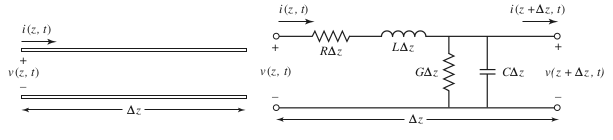
\includegraphics[scale=0.6]{circuitequivalent}
  \caption{Circuit equivalent d' una línia de transmissió}
  \label{fig:circuit}
  \vspace{-1 em}
\end{figure}

\subsection{Capacitat}

Els dos conductors de la línia formen un condensador amb càrrega $Q$ i tensió $V$, amb capacitància total $\mathcal C = \frac{Q}{V}$. Com que la cárrega és proporcional a la longitud de la guia $l$ podem definir la capacitat per unitat de longitud $C = \frac{\mathcal C}{l} = \frac{Q}{l V}$.

\subsection{Inductància}

Considerem el circuit rectangular format per dos línies al llarg dels conductors i dos linies entre els conductors a l' entrada i a l' eixida (vore figura). El flux a través d' aquesta secció del camp magnètic creat pels corrents als conductors forma una autoinductància $\mathcal L = \frac{\phi}{I}$, que al igual que la capacitància és proporcional a la longitud de la línia i dona lloc a una autoinductància distribuïda $L = \frac{\mathcal L}{l} = \frac{\phi{}}{l I}$

\subsection{Conductància}

Si el dielèctric té pèrdues, caracteritzades per $\epsilon _r $, $\sigma \sub D\neq \infty$, existirà una corrent de pèrdues en la direcció radial $\vec J = \sigma \sub D\vec E$. La conductància d' aquesta corrent és $\mathcal G = \frac{1}{R} = \frac{I \sub {pèrdues}}{V} = \frac{\int \vec J \sub{pèrdues} d \vec S}{V} = \frac{\int \sigma \sub D\vec E d \vec S}{V} = \frac{\sigma _D}{V} \int \vec E d \vec S$. Com que la integral és calcula sobre un cilindre concèntric als conductors tindrem $\mathcal G \propto l$, i definim $G = \frac{\mathcal G}{l}$

\subsection{Resistència}

Com que la conductància dels conductors és alta però no infinita tindrem pèrdues en aquests, determinades per la seua resistència superficial $R_s$. Sabem del tema anterior que les pèrdues han de ser $P_p = \frac{1}{2} R_s \int \vert \vec H \sub{sup} \vert dS$. Com que en teoria de circuits la potència dissipada per una resistència és $\frac{1}{2} \vert I \vert ^2 \mathcal R$, la resistència equivalent de la línia és $\mathcal R = \frac{R_s}{\vert I \vert ^2} \int \sub {cond} \vert \vec H  \vert dS$, i al ser la integral sobre els conductors proporcional a $l$ definim $R = \frac{\mathcal R}{l}$.

\section{Ones de tensió i corrent}

Cada element $\Delta z$ de la línia, per tant, pot ser tractat com un circuit amb dos fils (un per cada conductor) i el elements circuitals apropiats, com es mostra a la figura. L' ordre dels elements és irrellevant.

Ara podem utilitzar teoria de circuits per a estudiar el comportament de la diferència de potencial entre els dos conductors/fils $V(z, t)$ i la corrent que circula per aquests $I(z, t)$. Al llarg de $\Delta z$ els elements del circuit modificaran aquestes quantitats:
\begin{subequations}
  \begin{align}
    V(z) - V(z + \Delta z) &= I(z) (j L \omega \Delta z + R \Delta z) \\
    I(z) - I(z + \Delta z) &= V(z + \Delta z) (j \omega C \Delta z t + G \Delta z)
  \end{align}
\end{subequations}

Si dividim entre $\Delta z$ i fem el limit $\Delta z \to 0$ obtenim dues equacions diferencials acoblades, anomenades equacions del telègraf:
\begin{subequations}
  \begin{align}
    - \frac{dV}{dz} &= I(z)(j\omega L + R ) \label{diffV} \\
    - \frac{dI}{dz} &= V(z)(j\omega C + G )
  \end{align}
\end{subequations}

Definint $Z = R + j \omega L $ i $ Y = G + j \omega C$ i derivant ambdues entre $z$ les desacoblem i obtenim les solucions, que resulten ser dues ones.
\begin{subequations}
  \begin{align}
    V = V _0 e^{j \omega t}e^{\pm \sqrt{ZY} z} \label{solV}\\
    I = I _0 e^{j \omega t}e^{\pm \sqrt{ZY} z} \label{solI}
  \end{align}
\end{subequations}


\section{Relació entre tensió i corrent}

Si $V$ està relacionada amb $H$, $I$ està relacionada amb $\vec E$, i $\vec E$ amb $\vec H$, ha d' existir una relació entre $V$ i $I$. Substituint \cref{solV,solI} en \cref{diffV} obtenim
\begin{equation}
  \frac{V}{I} = \pm\sqrt{\frac{Z}{Y}} = \pm\sqrt{\frac{R+j\omega L}{G + j\omega C}} = \pm Z_c
\end{equation}
On $Z_c$ és una quantitat complexa amb dimensions de resistència, que s' anomena impedància característica de la línia, ja que sols depén de les propietats físiques d' aquesta. El signe positiu correspon a la $Z_c$ que afecta a la ona que viatja en el sentit $+z$, i el negatiu a la que va cap a $-z$. Si connectem dues línies la diferència entre les $Z_c$ pot provocar reflexions no desitjades, pel que totes les linies de transmissió operen a 50 $\Omega $.

\section{Factor de propagació}

El factor de propagació de les ones de tensió i corrent, $\gamma = \sqrt{ZY}$, és un número complex, les parts real i imaginària del qual estan relacionades amb l' atenuació exponencial i la ondulació, respectivament.
\begin{equation}
  \sqrt{ ZY }= \sqrt{(R + j \omega L)(G + j\omega C)} = \frac{\alpha}{2} + j \beta
\end{equation}

Estudiem aquests dos termes en casos importants.

\subsection{Línia sense pèrdues}

En una línia sense pèrdues $R = G = 0$, pel que $\gamma = \sqrt{j\omega Lj\omega C} = j\omega \sqrt{LC}$, i les ones tindran freqüència $\beta = \omega \sqrt{LC}$, i $v_f = v_g = \frac{1}{\sqrt{LC}}$. Aquestes línies tenen $Z_c = \sqrt{\frac{L}{C}}$.

\subsection{Línia amb poques pèrdues}

Si $R << \omega L$ i $G << \omega C $ podem obtindre una expressió aproximada per a les parts reals i imaginària de $\gamma$ expandint fins a segon ordre (si sols utilitzem primer ordre els resultats són els mateixos que en el cas anterior):
\begin{subequations}
  \begin{align}
   \gamma &= \sqrt{(R + j\omega L)(C + j\omega C)} = \sqrt{\frac{j\omega L }{j\omega C}}  \sqrt{\left ( 1 +  \frac{R}{j\omega L} \right) \left ( 1 + \frac{G}{j\omega C } \right )}  \\
   &\approx \frac{\sqrt{LC}}{2} \left ( \frac{R}{L} + \frac{G}{C} \right ) \left [ 1 - \frac{1}{8 \omega ^2} \left ( \frac{R}{L} - \frac{G}{C} \right ) ^2 \right ] + j \omega \sqrt{LC} \left [ 1 +  \frac{1}{8 \omega^2} \left ( \frac{R}{L} - \frac{G}{C} \right) ^2 \right ] \nonumber
  \end{align}
 
\end{subequations}

Com que la freqüència de la ona $\omega$ apareix als dos termes cada component freqüèncial de la ona tindrà una atenuació i una velocitat de propagació, pel que existirà dispersió. La impedància serà:
\begin{equation}
  Z_c = \sqrt{\frac{R + j \omega L}{G + j\omega C}} \approx \sqrt{\frac{L}{C}} \left [ 1 - \frac{j}{2 \omega } \left ( \frac{R}{L} - \frac{G}{C} \right) \right ]
\end{equation}

\subsection{Corrent continua DC}

En corrent continua  ($\omega = 0$), pel que  $\gamma = \sqrt{RG}$ i $Z_c = \sqrt{\frac{R}{G}}$. Quan treballem amb DC no solem percebre efectes ondulatoris perquè $G$ és prou xicoteta, per exemple al llarg dels cable del multímetre: com que els cables són curts apenes observem la caiguda de V, però si tinguèrem cables de 120 metres observariem ondulacions en les mesures.

\section{Comentaris}

\subsection{Alternatives per a calcular C, L i G}

Existeix un altra manera de clacular els paràmetres distribuïts C, L i G. A partir de les expressions per a la energia acumulada a un condensador i a una inductància en funció dels camps i de les expression en funció de $C$ i $L$:
\begin{subequations}
  \begin{align}
    \epsilon _c = \frac{1}{2} C V ^2 = \frac{1}{2} \int \vec E \vec D dV \to C &= \frac{1}{V^2} \int \vec E \vec D dV \\
    \epsilon _L = \frac{1}{2} L I ^2 = \frac{1}{2} \int \vec B \vec H dV \to L &= \frac{1}{I^2} \int \vec H \vec B dV
  \end{align}
\end{subequations}

Per a $G$ podem utilitzar la relació coneguda per a qualsevol condensador:
\begin{equation}
  \label{relCG}
  \frac{C}{G} = \frac{ \epsilon _ r \epsilon _0}{\sigma \sub D}
\end{equation}

\subsection{Paràmetres independents}

Per a una línia tenim quatre paràmetres distribuits, però són tots independents? Sabem que $v_g = \frac{1}{\sqrt{LC}}$ i que en TEM $v_g = \frac{1}{\sqrt{\mu\epsilon}}$, pel que $L$ i $C$ estan relacionats per $\sqrt{LC} = \sqrt{\mu \epsilon}$. També sabem que $C$ i $G$ están relacionats per \cref{relCG}. Per tant sols són independents $R$ i un altre paràmetre.

\subsection{Incertessa energia / temps}

Imaginem una ona sinusoidal a freqüència $\omega_0$ que viatja ca a $+z$. La TdF ens dona el seu espectre en freqüències, que és una delta en $\omega _ 0$. Sabem que arriba a algun lloc, però no quan arriba, ja que desde $t=-\infty$ fins a $t = \infty$ la ona existeix en tot l' espai. Per a poder parlar de quan comença o acaba hem de ``marcar-la'', i que dure de $t=a$ fins a $t=b$. Ara, però la TdF ja no és una delta, sino una campana de Gauss al voltant de $\omega _0$ amb amplitud inversament proporcional a $b - a$. Quan més localitzada està una ona menys s' aproxima a una freqüència pura.

 En les ones tenim dues incertesses com aquesta: freqüència-temps ( o energia-temps) i nombre d' ones - posició ( o moment - posició).

\chapter{Linies de transmissió carregades}

\section{Introducció}

Fins ara les línies eren infinites, però necessàriament ha d' haver un generador al principi i un dispositiu al final que reba les ones: equips de mesura, antenes, filtres, forns de microones... Aquestes discontinuïtats, anomenades càrregues, no donen problemes a freqüències baixes, però a altes poden provocar reflexions, pel que tindrem dues ones en la guia. En el circuit les representarem com a impedàncies (figura \cref{circeq})  En aquesta secció anomenarem $z=0$ al punt on la guia es connecta a la càrrega.
\begin{figure}[ht]
  \centering
  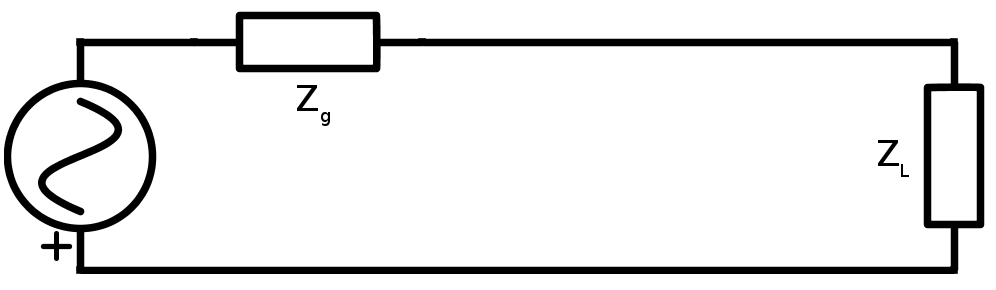
\includegraphics[scale=0.20]{circ0}
  \caption{Circuit equivalent a una guia carregada i amb generador}
  \label{circeq}
  \vspace{-2 em}
\end{figure}

\section{Coeficient de reflexió en la càrrega}

La impedància de la càrrega (vore figura \cref{genplusload})
\begin{equation}
  Z_L = \frac{V_L}{I_L} = \frac{V_0 ^+ + V_0 ^-}{I_0 ^+ + I_0 ^-}
\end{equation}
 está relacionada amb la de la ona
\begin{equation}
  Z_C = \frac{V_0 ^+}{I_0^+} = - \frac{V_0 ^-}{I_0 ^-}
\end{equation}
per el coeficient de reflexió $\Gamma = \frac{V_0 ^-}{V_0 ^+}$ seguint la relació $\Gamma = \frac{Z_L - Z_C}{Z_L + Z_C}$, pel que la fracció d' energia reflectida dependrà de la diferència entre $Z_L$ i $Z_C$. Com que mesurar impedàncies és complicat és preferible usar el $\Gamma $ per a estudiar els efectes de les càrregues.
\begin{figure}[ht]
  \centering
  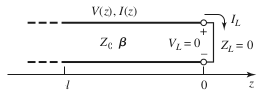
\includegraphics[scale=0.7]{loadint}
  \caption{Intensitat i voltatge en la càrrega}
  \label{genplusload}
\end{figure}

Observem que en un circuit obert, en que $Z_L = \infty$, tota l' ona és reflectida ($\Gamma = 1$) i en un curtcircuit, on $Z_L = 0$, la ona es reflexa canviada de fase ($\Gamma = -1$). En el cas en que la càrrega està adaptada a la guia $Z_L = Z_C$ tenim que $\Gamma = 0$, i és el cas òptim en que no existeixen reflexions. És per això que quasi totes les guies i dispositius tenen una impedància de $50 \Omega$.

\section{Potència consumida}

De la expressió per a la potència consumida per una resistència podem obtindre la potència consumida per la càrrega:
\begin{equation}
 \begin{split}
    P_L =& \frac{1}{2} \Re (V_L \cdot I_L ^*) = \frac{1}{2} \Re \left [ (\vp + \vm)(\ip + \im) \right]  \nonumber \\
  = &\frac{1}{2} \Re \left [ \vp (1+\Gamma _L) \left ( \frac{\vp}{Z_L} \right ) ^ * (1- \Gamma _L) \right] \nonumber \\
  = &\frac{1}{2} \abs \vp \Re \left [ \frac{1}{Z_C ^*}(1 - \abs{ \Gamma_L } ^2 + 2)\abs {\Gamma _L} ^2\sin \theta) \right]
  \end{split}
\end{equation}

Si $Z_C \in \Re$, com és el cas quan la guia té poques pèrdues, la podem deixar
\begin{equation}
  \label{eq:pot}
  P = \frac{1}{2} \frac{\abs \vp ^2}{Z_C} (1 - \abs {\Gamma_L} ^2)
\end{equation}

En aquesta expressió el primer terme és la potència que l' ona incident du cap endavant, mentre que el segon ens diu quin percentatge d' aquesta no és consumit per la càrrega.

\section{Ones estacionàries}

Quan dos ones viatjant en direccions oposades es superposen obtenim una ona estacionària:
\begin{subequations}
  \begin{align}
    V(z) = \vp \e{- \jmath \beta z} + \vm \e{ \jmath \beta z} \\
    I(z) = \ip \e{- \jmath \beta z} + \im \e{ \jmath \beta z}
  \end{align}
\end{subequations}

Per conveniència i conveni definim $\l = -z $, i reescrivim aquestes expressions com
\begin{subequations}
  \begin{align}
    V(\l) & = \vp \e{- \jmath \beta z} (1 + \Gamma _L \e{-\jmath 2 \beta z}) \nonumber \\
         & = \vp \e{ \jmath \beta \l} (1 + \abs {\Gamma _L} \e{\jmath (2 \beta \l + \theta)}) \\
    I(\l) &= \frac{\vp}{Z_L} \e{ -\jmath \beta z} (1 - \Gamma _L \e{-\jmath 2 \beta z}) \nonumber \\
\label{guideI}
         &= \frac{\vp}{Z_L} \e{ \jmath \beta \l} (1 - \abs{\Gamma _L} \e{\jmath (2 \beta \l + \theta)}) 
  \end{align}
\end{subequations}

\section{Impedància d' entrada d' una línia}

Així com en el punt $z = 0$ (el punt de la càrrega) hem definit $Z_L$ i $\Gamma _L$  a partir de $\vp$, $\vm$, ... podem fer el mateix en qualsevol punt de la línia, i definir del quocient de reflexió d' entrada entre les dues ones:
\begin{equation}
  \Gamma _{in} = \frac{V_z ^- }{V_z ^ +} = \frac{\vm \e{\jmath \beta z}}{\vp \e{-\jmath \beta z}} = \Gamma _L \e{\jmath 2 \beta z} = \abs { \Gamma _L } \e{- \jmath (\theta -2 \beta \l)}
\end{equation}

Continuant l' analogia podem definir la impedància d' entrada de la línia com el quocient
\begin{equation}
  Z_L = \frac{V(z)}{I(z)} = \frac{V^+ (z) + V^-(z)}{I^+(z) + I^- (z)} = Z_C \frac{V^+ (z) + V^-(z)}{V^+(z) - V^- (z)} = Z_C \frac{1+ \Gamma _{in}}{1 - \Gamma _{in}}
\end{equation}

La impedància d' entrada de la línia pot ser reescrita usant solament les propietats de la línia:
\begin{equation}
  Z_{in} = Z_C \frac{Z_L + Z_C \jmath \tan (\beta \l)}{Z_C + Z_L \jmath \tan (\beta \l)}
\end{equation}

La impedància puntual és per tant periòdica en $\frac{\lambda}{2}$, i quan $\beta \l = n\frac{\lambda}{2}$ és com si no hi haguera línia entre el punt $z$ i la càrrega $ Z_{in} = Z_L$, com en la figura \cref{imptoimp}.

\begin{figure}[ht]
  \centering
  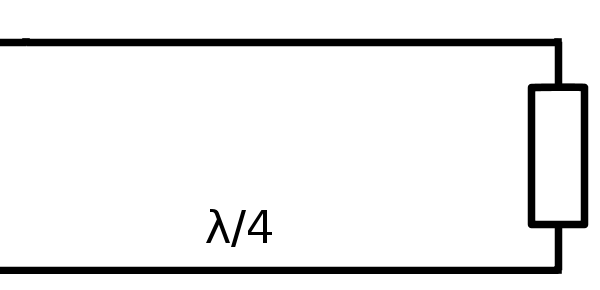
\includegraphics[scale=0.35]{impllarg}
  \quad
  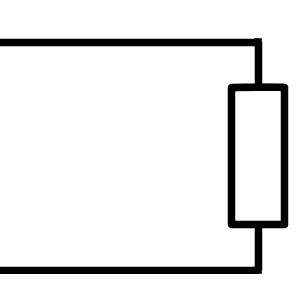
\includegraphics[scale=0.35]{impcurt}
  \caption{Impedàncies equivalents}
  \label{imptoimp}
\end{figure}

 Quan la línia és d' un quart d' ona, o $\l =  = \frac{\lambda}{4} + n \frac{\lambda}{2}$, el terme $\tan (\beta \l)$ es dispara a $\infty$, i la impedància és
\begin{equation}
  Z_{in} =  \frac{Z_C ^2}{Z_L}
\end{equation}

Una línia així s' anomena transformador de quart d' ona, perquè pot transformar la càrrega de diverses maneres. Si la càrrega és una inductància de valor $L$, la impedància en el punt $l$ serà igual a la d' un capacitador (vore figura \cref{indtocond}).
\begin{equation}
  Z_{in} = \frac{Z_C ^2}{jL\omega} = Z_{condensador}
\end{equation}

\begin{figure}[ht]
  \centering
  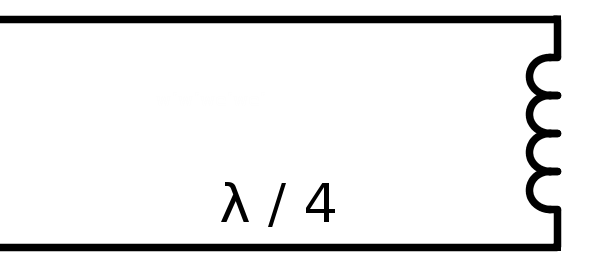
\includegraphics[scale=0.3]{inducllarg}
  \quad
  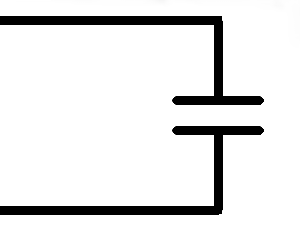
\includegraphics[scale=0.35]{condcurt}
  \caption{L' inductància i el transformador donen lloc a un capacitador}
  \label{indtocond}
\end{figure}

I si la càrrega és un capacitador, la impedància serà la d' una inductància (figura \cref{condtoind}) tindrem
\begin{equation}
  Z_{in} = j C \omega Z_C^2 = Z_{inductor}
\end{equation}

\begin{figure}[ht]
  \centering
  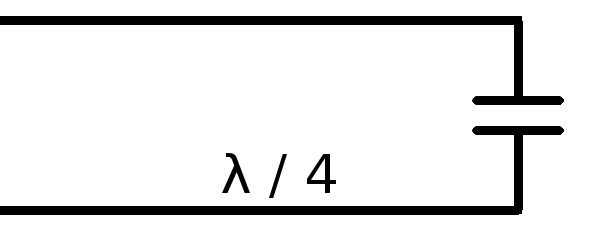
\includegraphics[scale=0.35]{condllarg}
  \quad
  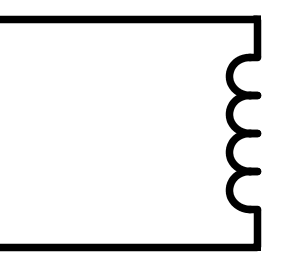
\includegraphics[scale=0.3]{induccurt}
  \caption{El condensador i el transformador donen lloc a un inductor}
  \label{condtoind}
\end{figure}

Com els inductors ''de llibre'' són difícils de construir podem utilitzar aquest resultat per a construir-los usant un condensador amb una guia de quart d' ona.

\section{Generador i línia}

Tots els anàlisis fets fins ara estan en funció de $\vp$, que depén del generador que alimenta la línia. Aquest està caracteritzat per tres variables: $V_g$, $\omega$ i $Z_g$. Relacionar $V_g$ i $V_0$, però, és complicat.

La càrrega i el segment de línia entre el generador i aquesta poden ser estudiats com una sola impedància (vore figura \cref{circeq})  per la que passa una corrent
\begin{equation}
  I_L = \frac{V_g}{Z_g + Z_{in}}
\end{equation}

Aquesta corrent ha de ser igual a la que corre per la guia \cref{guideI}, i igualant-les obtenim la relació entre els voltatges:
\begin{equation}
  I_L = I(l) \to \frac{V_g}{Z_g + Z_{in}} = \frac{\vp}{Z_C} \e{\jmath \beta \l} (1 - \Gamma _{in})
\end{equation}

I per tant
\begin{equation}
  \vp = V_g \e{- \jmath \beta \l} \frac{Z_C}{Z_g + Z_C + \Gamma _{in}(Z_C - Z_g)}
\end{equation}
pel que $\abs \vp = f(V_g, \l)$ i tenim el problema de que la potència consumida dependrà de la distància ( a través de $\Gamma_{in}$), el que seria inconvenient perquè ens obligaria a usar guies que foren múltiples d' una certa distància o perdre energia. El significat físic d' açò és que la ona torna a reflectir-se en el generador, i perdem energia.

Aquest problema ve de la presència de $\Gamma _{in}$ en l' expressió que relaciona $\vp$ i $V_g$. Una solució simple és assegurar-se de que $Z_C = Z_g$, i així
\begin{equation}
  \abs \vp = Z_C \frac{V_g \e{- \jmath \beta \l }}{Z_g + Z_C}
\end{equation}

Per conveni els generadors es fabriquen quasi sempre de manera que la $Z_g$ siga de 50 $\Omega$, igual que les guies. El desavantatge és que la impedància interior del generador consumirà energia, però és preferible.

\chapter{Guies tancades homogènies}

\section{Introducció}

A diferència de les línies de transmissió, que tenien dos conductors, les línies de transmissió estan formades per un sol conductor, el que impedeix que propaguen el mode $TEM$ però facilita la transmissió de $TE$ i $TM$ (i de modes híbrids, que no vorem). Com que l' únic mode que no té freqüència de tall és el $TEM$ no podrem utilitzar-les per a conduir DC, però poden transportar més potència per unitat d' àrea seccional. Com que no propaguen $TEM$, tindrem sempre components axials, i com que la velocitat de propagació $\beta = \sqrt{\omega ^2 \mu\epsilon - k_c ^2}$ no és lineal seran inherentment dispersives.

\section{Guia rectangular}

La guia rectangular (figura \cref{rectangular}) és un disseny senzill d' estudiar i que té amples aplicacions. Suporta $TE$ i $TM$. Per a obtindre els camps en aquesta guia, per exemple en el mode $TM$, hem de resoldre la equació de Helmholtz
\begin{equation}
  \label{ezhelm}
  \del _t \vec e_z + (k^2 - \beta ^2) \vec e_z = 0
\end{equation}
per a obtindre $\vec e_z$ i $\beta$ , i a partir d' aquests podem obtenir els altres camps usant
\begin{figure}%[ht]
  \centering
  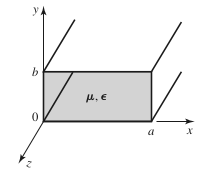
\includegraphics[scale=0.6]{rectangular}
  \caption{Guia d' ona rectangular}
  \label{rectangular}
  \vspace{-1 em}
\end{figure}

\begin{equation}
  \label{otherfields}
  \vec e_t = \frac{- \jmath \beta}{k^2 - \beta ^2} \del _t  e_z \quad i \quad \vec h_t = Y_{TM} \uz \times \vec e_t
\end{equation}

Resolent \cref{ezhelm} per separació de les variables $x$ i $y$ obtenim
\begin{equation}
  e_z = \left[ A \cos (k_x x ) + B \sin (k_x x) \right ] \left[ C \cos(k_y y ) + Dsin(k_y y) \right]
\end{equation}

On $k_x ^2 + k_y ^2 = k^2 - \beta ^2$. Per a calcular $\beta$ usar les condicions de contorn, que són
\begin{equation}
  e_z(x = a) = e_z (x = 0) = e_z(y = b) e_z(y = 0) = 0
\end{equation}

De les dos primeres obtenim que $A = 0$ i $k_X = \frac{n \pi}{a}$, i de les dos segones $C = 0$ i $k_y = \frac{m \pi}{b}$, el que ens deixa
\begin{equation}
  \label{solez}
  e_z (x, y) = BD \sin \frac{n \pi}{a} \sin \frac{m \pi }{b} = E_0  \sin \frac{n \pi}{a} \sin \frac{m \pi }{b}
\end{equation}

on hem reanomenat el coeficient $BD$ com a $E_0$, i
\begin{equation}
  \label{eq:solbeta}
  \beta_{nm} = \sqrt{ \omega ^2 \mu \epsilon - k_x ^2 - k_y ^ 2 } = \sqrt{\omega^2 \mu \epsilon - \left (\frac{n \pi}{a} \right ) ^2 - \left ( \frac{m \pi}{b} \right) ^2 }
\end{equation}

Per a cada parella $(n, m)$ existeix una solució, o el que és el mateix, un mode $TM_{nm}$, (excepte per al cas $n=m=0$, ja que seria la solució trivial en que no hi ha camps). Per a que aquests modes es propaguen $\beta $ haurà de ser real, el que implica
\begin{equation}
  \label{conds}
  \omega ^2 \mu \epsilon >  \left (\frac{n \pi}{a} \right ) ^2  + \left ( \frac{m \pi}{b} \right) ^2
\end{equation}

Definim per tant la freqüència de tall del mode $TM_{nm}$ com
\begin{equation}
  \omega _{c \,nm} =  \frac{1}{\sqrt{\mu \epsilon}} \sqrt{   \left (\frac{n \pi}{a} \right ) ^2 + \left ( \frac{m \pi}{b} \right) ^2}
\end{equation}

on s' observa que a freqüències més altes més modes seran propagables. La resta de camps poden obtindre's usant \cref{otherfields}:
\begin{subequations}
\begin{align}
  \vec e_t = \frac{ - \jmath \beta }{k^ 2 - \beta ^ 2} E_0
  \bigg [
    &+\left (\frac{n \pi}{a} \cos \frac{n \pi x}{a} \sin \frac{m \pi y}{b} \right ) \ux \nonumber \\
    &+\left (\frac{m \pi}{b} \sin \frac{n \pi x}{a} \cos \frac{m \pi y}{b} \right )\uy
  \bigg ] \\
  \vec h _ t = \frac{  -\jmath \omega \epsilon }{k^ 2 - \beta ^ 2} E_0
  \bigg [
    &-\left (\frac{m \pi}{b} \sin \frac{n \pi x}{a} \cos \frac{m \pi y}{b} \right ) \ux \nonumber \\
    &+\left (\frac{n \pi}{a} \cos \frac{n \pi x}{a} \sin \frac{m \pi y}{b} \right ) \uy
  \bigg ]
\end{align}
\label{rectTM}
\end{subequations}

El procediment amd els modes $TE$ és anàleg, usant les condicions de contorn
\begin{equation}
  \vec h_t = 0 \to \left. \del h_z \right \vert \sub{parets} = 0 \to \left. \pd{h_z}{x}  \right \vert \sub{par} =  \left. \pd{h_z}{y}  \right \vert \sub{par} = 0
\end{equation}
obtenim
\begin{equation}
  h_z = H_0 \cos \left ( \frac{n \pi x}{a} \right ) \cos \left ( \frac{m \pi y}{b} \right )
\end{equation}
\begin{subequations}
\begin{align}
  \vec h_t = \frac{  \jmath \beta }{k^ 2 - \beta ^ 2} H_0
  \bigg [
    &+\left (\frac{n \pi}{a} \sin \frac{n \pi x}{a} \cos \frac{m \pi y}{b} \right ) \ux + \nonumber \\
    &+\left ( \frac{m \pi }{b} \cos \frac{n \pi x}{a} \sin \frac{m \pi y}{b} \right ) \uy
  \bigg ] \\
  \vec e _ t = \frac{  \jmath \omega \mu }{k^ 2 - \beta ^ 2} H_0
  \bigg [
    &+\left (\frac{m \pi}{b} \cos \frac{n \pi x}{a} \sin \frac{m \pi y}{b} \right ) \ux \nonumber \\
   &-\left ( \frac{n \pi }{a} \sin \frac{n \pi x}{a} \cos \frac{m \pi y}{b} \right ) \uy 
  \bigg ]
\end{align}
\end{subequations}

amb
\begin{equation}
  \beta = \sqrt{ \omega ^2 \mu \epsilon - k_x ^2 - k_y ^ 2 } = \sqrt{\omega^2 \mu \epsilon - \left (\frac{n \pi}{a} \right ) ^2  - \left ( \frac{m \pi}{b} \right) ^2 }
\end{equation}
\begin{equation}
  \omega _{c \,nm} =  \frac{1}{\sqrt{\mu \epsilon}} \sqrt{   \left (\frac{n \pi}{a} \right ) ^2 + \left ( \frac{m \pi}{b} \right) ^2}
\end{equation}

\begin{figure}[ht]
\begin{minipage}{8cm}
  \centering
  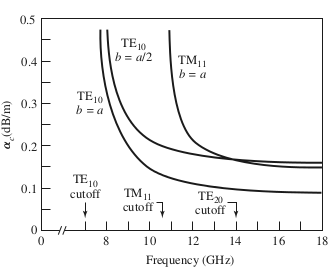
\includegraphics[scale=0.5]{rectangularmodes}
  \caption{Atenuació de modes en una guia rectangular}
  \vspace{-1 em}
\end{minipage}
\begin{minipage}{8cm}
  \centering
  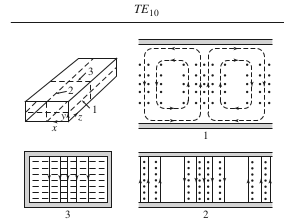
\includegraphics[scale=0.6]{rectangularfundamental}
  \caption{Mode fonamental d' una ona rectangular}
  \label{rectangularfundamental}
  \vspace{-1 em}
\end{minipage}
\end{figure}

\section{Mode fonamental}

El mode fonamental és aquell que es propaga amb la menor freqüència de tall. En el cas de la guia rectangular és el $TE_{10}$, graficat en la figura \cref{rectangularfundamental}
\begin{equation}
  \vec E = - H_0 \frac{\jmath \omega \mu a}{\pi} \sin \left ( \frac{\pi}{a} x \right) \uy
\end{equation}
\begin{equation}
  \vec H =  H_0 \left[\frac{\jmath \beta a}{\pi} \sin \left ( \frac{\pi}{a} x \right) \ux + \cos \left ( \frac{\pi}{a} x \right ) \uz \right]
\end{equation}

\section{Guia circular}

Usarem la guia circular (figura \cref{circular}) per a il·lustrar el cas en que la simetria fa preferible utilitzar coordenades no cartesianes, en aquest cas les cilíndriques $(s, \varphi, z)$.

Per a trobar els modes $TM_{nm}$ resolem, com abans, l' equació de Helmholtz, però aquesta vegada usant el Laplacià en coordenades cilíndriques:
\begin{equation}
  \del _t ^ 2 e_z + (k^ 2 - \beta ^2 ) e_z = \left ( \pd[2]{}{s} + \frac{1}{s}\pd{}{s} + \frac{1}{s^2} \pd[2]{}{\varphi}  \right )  e_z + k_c ^2 e_z
\end{equation}

\begin{figure}[ht]
  \centering
  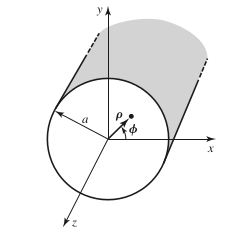
\includegraphics[scale=0.4]{circular}
  \caption{Guia d' ona circular}
  \label{circular}
  \vspace{-1 em}
\end{figure}

Separant $e_z$ en $R(s)\Phi(\varphi)$ arribem a dues equacions:
\begin{equation}
  \frac{s^2}{R(s)} \pd[2]{R}{s} + \frac{s}{R(s)} \pd{R}{s} + (k^2 - \beta ^2) s^2  =
  \frac{1}{\Phi(\varphi)} \pd[2]{\Phi}{\varphi} =
  k_{\varphi} ^2
\end{equation}

Ls solucions de la part angular són simples:
\begin{equation}
  \label{solangular}
  \Phi (\varphi) = A \cos(k _{\varphi} \varphi ) + B \sin (k_{\varphi} \varphi)
\end{equation}
però les de la part radial són més complicades; són funcions de Bessel primer i segon espècie:
\begin{subequations}
  \begin{align}
    R(s) = \Bf _{k_\varphi} (s\sqrt{k^2 - \beta ^2})  =  \Bf _{k_\varphi} (s k_c)  \nonumber \\
    R(s) = \Bs _{k_\varphi} (s\sqrt{k^2 - \beta ^2})  =  \Bs _{k_\varphi} (s k_c)  \nonumber
  \end{align}
\end{subequations}

Com que el camp ha de ser continuu en la coordenada angular tenim la condició de contorn
\begin{equation}
  e_z(\varphi = \alpha) = e_z ( \varphi = \alpha + 2 \pi l) \quad \forall \alpha \quad \forall l \in \Nat
\end{equation}

que, introduïda en \cref{solangular} ens diu que $k_{\varphi} \in \Zahl$:
\begin{equation}
  \Phi (\varphi ) = A \cos (n \varphi ) + B \sin (n \varphi)
\end{equation}

En quant a la part radial, en $s = 0$ les funcions de Bessel de segon espècie $\Bs$ divergeixen, pel que $D = 0$, i la condició de contorn de les parets $e_z(s = 0) = a$, que ha de cumplir-se $\forall \varphi$ ens dona el valor de $k_c$ per al mode $n$: és la solució de
\begin{equation}
  \Bf _ n (k_c a ) = 0
\end{equation}

Com que les funcions $\Bf$ no tenen arrels analítiques haurem d' utilitzar taules o procediments numèrics per trobar-les. Denotarem la $m$-èsima arrel de $\Bf$ com a $P_{nm}$, i per tant $k_c = \frac{P_{nm}}{a}$. La solució final, doncs, és (anomenem $AC = E$ i $BC = F$):
\begin{equation}
  e_z = E \cos (n \varphi ) \Bf _n ( \frac{P_{nm}}{a} s ) + F \sin (n \varphi ) \Bf_n (\frac{P_{nm}}{a}s)
\end{equation}
amb $ \beta = \sqrt{\omega ^ 2 \mu \epsilon - \left ( \frac{P_{nm}}{a} \right ) ^2}$.

Tenim dos coeficients independents perquè hi ha dos graus de llibertat al sistema: la energia de la ona i la polarització d' aquesta. Rotant el sistema de coordenades podem fer zero una o l' altra. Obtindre la resta dels camps, com abans, és un procediment mecànic:
\begin{subequations}
  \begin{align}
    \vec e_t =& -\frac{\jmath \beta}{k^2 - \beta ^2} \del _t  e_z =  \vec e_t = \frac{- \jmath \beta}{k^2 - \beta ^2} \left ( \pd{ e_z}{s} \us + \frac{1}{s} \pd{e_z}{\varphi} \uf \right ) \nonumber \\
    =& \left(-\frac{ \jmath \beta}{k_c} \left [ E \cos (n \varphi) + F \sin (n \varphi) \right ] \Bf _n ' \left( \frac{P_{nm}}{a} s \right) \right) \us  \nonumber\\
     & \left(-\frac{ \jmath \beta }{k_c ^2 } \frac{n}{s} \left [ E \sin (n \varphi) - F \cos (n \varphi) \right ] \Bf _n \left(\frac{P_{nm}}{a} s \right) \right) \uf \\
    \vec h_t =& \, Y_{TM} \uz \times \vec e_t \nonumber \\
    =& \left( -\frac{ \jmath \omega \epsilon}{k_c^2} \frac{n}{s} \left [ E \sin (n \varphi) - F \cos (n \varphi) \right ] \Bf _n \left( \frac{P_{nm}}{a} s \right) \right) \us  \nonumber \\
     & \left (-\frac{ \jmath \omega \epsilon }{k_c } \left [ E \cos (n \varphi) + F \sin (n \varphi) \right ] \Bf _n '\left(\frac{P_{nm}}{a} s \right) \right ) \uf
  \end{align}
  \label{circTM}
\end{subequations}

\begin{figure}[ht]
\begin{minipage}{8cm}
  \centering
  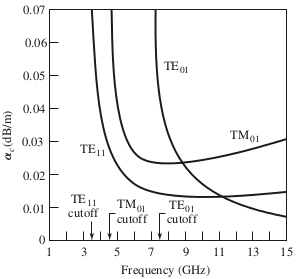
\includegraphics[scale=0.5]{circularmodes}
  \caption{Modes en una guia circular}
  \vspace{-1 em}
\end{minipage}
\begin{minipage}{8cm}
  \centering
  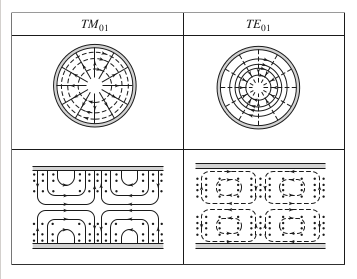
\includegraphics[scale=0.5]{circularmodesshape}
  \caption{Modes en una guia circular}
  \vspace{-1 em}
\end{minipage}
\end{figure}

\section{Guia coaxial}

La guia coaxial és una línia de transmissió que té moltes aplicacions gràcies al seu gran ample de banda, la seua baixa atenuació, i la capacitat de protegir les senyals propagades d' interferències exterior. En principi està dissenyada per a transmetre modes $TEM$, i podem utilitzar l' anàlisis del capítol 2, però és interessant estudiar el comportament dels camps d' aquesta quan transporta modes $TE$ o $TM$, ja que de vegades és inevitable que aquests modes apareguen junt al $TEM$ quan treballem amb freqüències altes (superiors a la del mode fonamental) o quan hi ha discontinuïtats, i és necessari saber com evitar interferències.

\begin{figure}[ht]
  \centering
  \begin{minipage}{7cm}
    \centering
    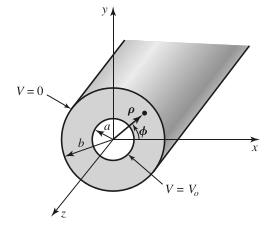
\includegraphics[scale=0.4]{coaxial}
    \caption{Guia d' ona coaxial}
    \label{coaxial}
  \end{minipage}
  \begin{minipage}{7cm}
    \centering
    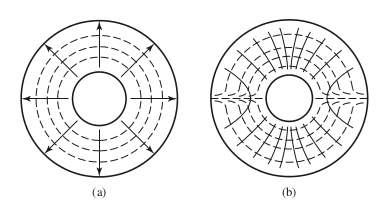
\includegraphics[scale=0.4]{coaxialmodes}
    \caption{Modes en una ona coaxial}
  \end{minipage}
\end{figure}

Quan apareixen aquestes discontinuïtats? Quan una guia s' estreta pot donar-se el cas que el mode fonamental es talle més enllà d' aquest punt, i la energia de la ona es reflectisca. Si després d' una distància curta l guia es torna a eixamplar és possible que el mode fonamental original torne a propagar-se. Que estiga tallat vol dir que s' atenua exponencialment, així que si no hi ha suficient distància per a que s' extingisca completament existirà un camp harmònic al final de la discontinuïtat, com si hi haguera un generador \footnote{En termes de fotons aquestes dos situacions són equivalents a un fotó rebotant contra una pared potencial infinita i fent efecte tunel, respectivament.}. Aquest fenomen pot ser usat per a excitar cavitats: necessitem fer entrar una ona en una regió tancada, però si fem un forat massa gran la cavitat tindrà massa pèrdues.

\subsection{Modes TE}

Com en el cas anterior comencem resolent l' equació de Helmholtz per a $h_z$ en coordenades cilíndriques, i després obtenim $\vec h_t$, $\vec e_t$ i $\beta$. Les solucions per a $h_z$ són, com abans,
\begin{equation}
  \Phi = A \cos ( n \varphi) + B \sin (n \varphi)
\end{equation}
\begin{equation}
  R = C \Bf_n ( k_c s ) + D \Bs_n (k_c s)
\end{equation}


On ja hem aplicat la continuïtat de la coordenada angular $\Phi(\varphi) = \Phi(\varphi + 2\pi l)$. Ara, però, no podem utilitzar la condició de contorn en $s = 0$ que hem utilitzat amb la guia circular, ja que ara el punt $s = 0$ no és part del problema, i $\Bs$ no divergeix. Per a traure els coeficients usarem les condicions de continuïtat de $h_t$ a les parets: la component radial ha d' anul·lar-se a les parets. Com que $h_t \propto \del h_z$ podem dir que
\begin{equation}
   \left. \pd{h_z}{s} \right \vert \sub{parets} = 0 \quad \to \quad \left. \pd{R}{s} \right \vert \sub{s = a} = \left. \pd{R}{s} \right \vert \sub{s = b} = 0
\end{equation}

Amb el que arribem a un sistema d' equacions en les incògnites C i D
\begin{equation}
  C\Bf _n ' (k_c a) + D \Bs _ n ' (k_c a) = 0
\end{equation}
\begin{equation}
  C\Bf _n ' (k_c b) + D \Bs _ n ' (k_c b) = 0
\end{equation}

Per a que existisca una solució el determinant de la matriu de coeficients ha de ser zero, i per tant hem de tindre
\begin{equation}
  \Bf _n ' (k_c a) \Bs _n ' (k_c b ) - \Bf _n ' (k_c b) \Bs _n ' (k_c a) = 0
\end{equation}

Cada solució numèrica $m$ d' aquesta equació transcendental proporciona, per al mode $n$, una $k_{c\,nm}$. Els coeficients $C$ i $D$ no són independents; estan lligats per
\begin{equation}
  \frac{C}{D} = -\frac{\Bf _n ' (k_c b )}{\Bs _n ' (k_c b )} = -\frac{\Bf _n ' (k_c a )}{\Bs _n ' (k_c a )}
\end{equation}

La solució per al camp axial queda
\begin{equation}
  h_z = [A \cos (n \varphi) + B \sin (n \varphi) ][C \Bf _n ' (k_c \varphi) + D \Bs _n ' (k_c \varphi)]
\end{equation}

i els camps transversals es poden obtenir pel mètode habitual.


\section*{Nota}

Pareix que sempre que utilitzem coordenades cilíndriques pugam utilitzar la condició de continuïtat de $\varphi$, però en realitat no és questió del sistema de coordenades utilitzat, sino de la guia, que té simetria angular. Hi ha casos en que no hi ha aquesta simetria, per exemple en una guia amb secció en forma de "formatget". En aquest cas, però, tindriem CC en $\varphi=0$ i $\varphi = \alpha$.

\chapter{Guies superficials}

\section{Introducció}

En algunes situacions els camps electromagnètics estan "confinats" a una superfície; poden propagar-se en el pla d' aquesta, però s' atenuen exponencialment en la direcció ortogonal. Aquesta superfície sol ser la interfase entre dos dielèctrics, com en les guies integrades o les fibres òptiques.

\section{Làmina dielèctrica sobre plans de terra}

A la imatge \ref{slab} es mostra la geometria d' una làmina dielèctrica sobre un pla de terra (\textit{grounded slab}) i el sistema de coordenades utilitzat. Suposem que el dielèctric s' estén en $\inf < x < \inf$ i en $0 < z < \inf$, el que implica que els camps no tindran variació en la direcció $x$.

\begin{figure}[ht]
  \centering
  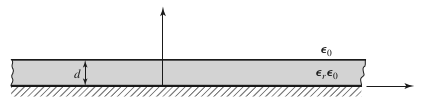
\includegraphics[scale=.6]{slabgeom}
  \caption{Làmina dielèctrica sobre terra}
  \label{slab}
\end{figure}

\subsection{Modes TM}

Comencem, com sempre, per resoldre la equació de Helmholtz per a $e_z$:

\begin{equation}
  \del _t \vec e_z + (k^2 - \beta ^2) \vec e_z = 0
\end{equation}
amb la particularitat de que $k^2 = \omega^2 \mu_0\epsilon _0$ en aire i $k^2 = \omega^2 \mu_0 \epsilon _0 \epsilon _r$ en el substrat, pel que tindrem dues regions separades, amb solucions diferents. Anomenant $k_c ^2 = k_0 ^2 \epsilon _r - \beta^2$ i $-h^2=k_0^2 - \beta^2$ tenim dues equacions diferencials

\begin{subequations}
  \begin{align}
    \pd[2]{e_z}{y} + k^2 _c e_z &= 0 \\
    \pd[2]{e_z}{y} - h^2 _c e_z &= 0
  \end{align}
\end{subequations}

Amb solucions

\begin{subequations}
  \begin{align}
    e_z &= A \cos(k_cy) + B \sin (k_c y) \quad \text{per a } y < d \label{yltd} \\
    e_z &= C \e{-hy} + D \e{hy} \quad \text{per a} y > d \label{ygtd}
  \end{align}
\end{subequations}

Per a que les condicions de contorn en la interfície aire - guia es satisfacin cal que les velocitats de fase siguen iguals, pel que la $\beta$ serà igual a les dues regions, i de $\beta^2 = k_0^2 \epsilon _r - k_c ^2 = k_o^2 - h^2$ obtenim 

\begin{equation}
  k_c^2 + h^2 = k_0 ^2 (\epsilon _r - 1)
  \label{final1}
\end{equation}

Usem les condicions de contorn

\begin{enumerate}
  \item{ $e_z < \infty$ quan $y \to \infty$, pel que $D$ ha de ser $0$ en \cref{ygtd}}
  \item{$e_z = 0$ quan $y=0$, d' on traguem $A = 0$ en \cref{yltd}.}
  \item{$e_z$ ha de ser continuu en $y=d$, donant lloc a la lligadura entre C i B
  \begin{equation}
    C \e{-hd}=B\sin(k_c d) \label{contin1}
  \end{equation}}
  \item{$\vec h_x$ ha der ser continuu en $y=d$. Com que $h_x = \frac{1}{\beta^2 - k^2}\pd{e_z}{y}$ tenim que
  \begin{equation}
   \left. \frac{-1}{h ^2} \pd{e_x}{y} \right \vert _{y = d^+} = \left . \frac{\epsilon _r}{k_c ^2} \pd{e_x}{y} \right \vert _{y = d^-}
  \end{equation}
  i, per tant,
  \begin{equation}
    \frac{1}{h} C e^{-hd} = \frac{\epsilon _r}{k_c ^2} B k_c \cos (k_c y) \label{contin2}
  \end{equation}
  }
\end{enumerate}

Les equacions \cref{contin1,contin2} formen un sistema d' equacions per a B i D. Per a que existisquen solucions el determinant ha d' anular-se:

\begin{equation}
  k_c \tan (k_c d) = h \epsilon_r
  \label{final2}
\end{equation}

Ara podem obtindre solucions per a $k_c$ i $h$ a partir de solucions numèriques per a les equacions \cref{final1,final2}. Si multipliquem ambdues per $d$ obtenim dues equacions 

\begin{subequations}
  \begin{align}
    (k_c d) \tan (k_c d) = (h d ) \epsilon _r \\
    (hd)^2 + (k_c d ) ^2 = (k_c d) ^2 ( \epsilon _r - 1 )
  \end{align}
\end{subequations}

que podem representar en el pla $hd$, $k_c$ (figura \cref{slabsolutions}). Notem que la segona de les equacions és un cercle de radi $k_0 d \sqrt{\epsilon - 1} = \omega d \sqrt{\mu \epsilon}\sqrt{\epsilon - 1}  $, i a major freqüència més interseccions tindrà amb les branques de la primera equació, el que significa que existiran més modes a la làmina. 

\begin{figure}[ht]
  \centering
  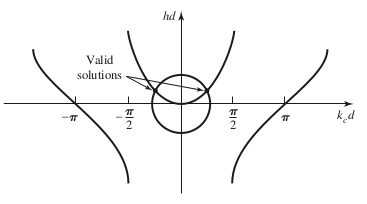
\includegraphics[scale=0.7]{slabsolutions}
  \caption{Sol·lucions gràfiques per a $k_c$ i $h$}
  \label{slabsolutions}
\end{figure}

Notem que el mode $TM_0$ no té freqüència de tall: és propaga desde $\omega= 0$ fins a $\omega = \infty$, encara que en $\omega = 0$ els camps desapareixen, el que resol la paradoxa que tindríem si tinguérem DC ($\omega = 0$) propagant-se amb un sol conductor.

Si la freqüència és molt gran les $h$ també ho seran, i el camp en $z$ s' atenuarà en una longitud $\sim \lambda$, pel que el camp estarà contingut al dielèctric \footnote{En una làmina amb més dielèctrics el camp es quedaria contingut al de major $\epsilon_r$}.

Els components restants es calculen mecànicament una vegada coneixem el valor de $h$ i $k_c$:

\begin{align}
  e_z &=  \begin{cases}
    B \sin (k_c y) & \text{quan }  y < d \\
    B \sin (k_c d) e^{-h(y - d)} & \text{quan } y > d
   \end{cases}\\
   \nonumber \\
  \vec e_t &= \begin{cases}
    \frac{\jmath \beta}{k_c} B \cos (k_c d)  \uy  & \text{quan }  y < d \\
    \frac{\jmath \beta}{h} B \sin (k_c d) e^{-h (y - d)} \uy & \text{quan } y > d
  \end{cases} \\
   \nonumber \\
  \vec h_t &= \begin{cases}
    \frac{\jmath \omega \epsilon_0 \epsilon_r}{k_c} B \cos (k_c y)  \uy & \text{quan } y < d \\
    \frac{\jmath \omega \epsilon_0}{h} B \sin (k_c d) e^{-h (y - d)} \ux & \text{quan } y > d 
  \end{cases}  \\
   \nonumber 
\end{align} 

\chapter{Ressonadors electromagnètics}

\section{Introducció}

Un ressonador és bàsicament una caixa de la que les ones no poden eixir, acumulant-se l' energia. Les ones interferiran amb les seues reflexions a les parets, pel que certes freqüències tenen ressonància. Aquest fenomen té moltes aplicacions: filtres freqüencials, emmagatzematge d' energia, forns de microones, acceleradors de partícules...

\section{Paràmetres d' un ressonador}

\begin{wrapfigure}{r}{7cm}
 % \centering
  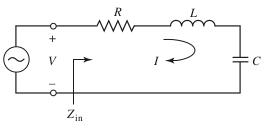
\includegraphics[scale=0.5]{RLCres}
  \caption{Circuit RCL equivalent}
  \label{RCLc}
\end{wrapfigure}

Un ressonador pot modelar-se com un circuit RCL (figura \cref{RCLc}), i està caracteritzat per els paràmetres d' aquest: la resistència, la inducció, la capacitat i el voltatge d' entrada.

La corrent d' aquest circuit és
\begin{equation}
  I_g = \frac{V_g}{R + \jmath \left (L \omega - \frac{1}{c\omega} \right)}
\end{equation}
Coneixent aquests paràmetres podem obtindre la potència generada (que és la mateixa dissipada per la resistència):
\begin{equation}
  P_g = P_R = \frac{1}{2}R \abs{I} ^2 = \frac{\frac{1}{2} R \abs{ V_g} ^2}{R^2 + \left(L \omega - \frac{1}{c\omega} \right)^2}
  \label{potg}
\end{equation}

\subsection{Freqüència de ressonància}

La corba de \cref{potg} és alta per a freqüències al voltant d' un valor $\omega _0$ que fa que el denominador siga mínim:
\begin{equation}
L \omega_0 - \frac{1}{C\omega _0} = 0 \to \omega _0 = \frac{1}{\sqrt{LC}}
\end{equation}

i baixa per a freqüències allunyades d' aquest valor, com es mostra a la figura \cref{potplot}.

\begin{figure}[ht]
  \centering
  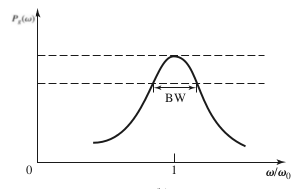
\includegraphics[scale=0.5]{poweroutput}
  \caption{Potència d' eixida d' un generador}
  \label{potplot}
\end{figure} 

L' amplada d' aquesta corba està caracteritzada pel factor de qualitat $Q$, definit com a 
\begin{equation}
  Q = \frac{\omega _ 0 }{\omega _2 - \omega _1}
\end{equation}

per a $\omega_2 > \omega _1$ tal que
\begin{equation}
P_g(\omega_2) = P_g (\omega _1 ) = \frac{1}{2} P_max = \frac{1}{2} \left ( \frac{1}{2} \frac{\abs{V_g} ^2}{R} \right ) 
\end{equation}

Quan més alt és $Q$ més selectiu és el filtre (menor ample de banda $BW$). Si resolem

\begin{equation}
P_g(\omega) = \frac{1}{2} P_max \to \frac{1}{4}\frac{\abs{V_g} ^2}{R} = \frac{\frac{1}{2} R \abs{ V_g} ^2}{R^2 + \left(L \omega - \frac{1}{c\omega} \right)^2}
\end{equation}
arribem al valor aproximat 
\begin{equation}
  (\omega - \omega_0) \sim \pm \frac{1}{2}\frac{R}{L} \to 
  \left\{ 
  \begin{array}{lr}
    \omega _2 = \omega _0 + \frac{1}{2}\frac{R}{L} \\
    \omega _1 = \omega _0 - \frac{1}{2}\frac{R}{L} 
  \end{array}
  \right.
\end{equation}

Pel que $\omega_2 - \omega_1 = \frac{R}{L}$ i $Q = \frac{\omega _0}{\omega_2 \omega _1} = \omega _0 \frac{L}{R} = \sqrt{\frac{L}{C}}\frac{1}{R}$

\subsection{Energia emmagatzemada}

La inductància i el condensador del circuit emmagatzemen energia, mentre que la resistència en perd. El quocient entre la energia emmagatzemada i la perduda és
\begin{equation}
  \frac{E_{emm}}{E_{per}} = \frac{\langle \frac{1}{2} L \abs{I} ^2 \rangle + \langle \frac{1}{2} C \abs{V} ^2 }{\frac{1}{2} R \abs{I} ^2} \rangle = \frac{\frac{1}{2} \frac{1}{2} L \abs{I} ^2  + \frac{1}{2} \frac{1}{2} C \abs{V} ^2 }{\frac{1}{2} R \abs{I} ^2} = \frac{L \abs{I} ^2 + C \frac{\abs{I}^2}{C^2 \omega^2}}{2 R \abs{I} ^2}
\end{equation}

On $\langle \cdot \rangle$ indica mitjana temporal. En el cas $\omega = \omega _0$ aquest coeficient és $\frac{L}{R}$, i vegem, i comparant-lo amb el factor de qualitat $Q = \omega _0 \frac{L}{R}$ descobrim que aquest també ens informa de la qualitat del ressonador com a emmagatzemador d' energia.

\subsection{Càlcul de Q en guies}

Per a calcular el factor $Q$ d' una guia d' ones usant $Q = \omega _0 \frac{\epsilon(\omega _0)}{P_l(\omega_0)}$ si coneixem la seua freqüència de ressonància $\omega _0$, la energia emmagatzemada $E_{stored} (\omega_0)$ i la potència perduda $P_{lost} (\omega _0)$. Aquesta última pot separa-se en dos contribucions: les pèrdues del conductor $P_{l,cond}$ i les del dielètric $P_{l,diel}$, i fer:
\begin{equation}
Q = \omega _0 \frac{E_s}{P_{l,c} + P_{l,d}} = \left [ \frac{P_{l`c}}{\omega_0 E_s }+\frac{P_{l`c}}{\omega _0 E_s} \right ] ^{-1} = \left [ \frac{1}{Q_D }+\frac{1}{Q_C} \right ] ^{-1}
\end{equation}

\subsubsection*{$Q$ d' un dielèctric}

La energia emmagatzemada en un dielèctric, en funció dels camps magnètics al seu interior, és
\begin{equation}
E_s = E_s(\vec E) + E_S(\vec H) = \frac{1}{2}\frac{1}{2} \int \vec E \cdot \vec D ^{*} dV + \frac{1}{2}\frac{1}{2} \int \vec H \vec B ^{*}dV = \frac{1}{2} \int \vec E \cdot \vec D^{*} dV = \frac{1}{2} \int \vec H \vec B ^{*} dV
\end{equation}

On hem utilitzat que en camps no atenuats la energia emmagatzemada pels camps elèctrics i magnètics és la mateixa. La potència perduda és
\begin{equation}
P_{l`d} = \frac{1}{2} \int \vec E \cdot \vec J ^{*} dV = \frac{\sigma_D}{2} \int \vec E \cdot \vec E ^{*} dV
\end{equation}
I per tant el factor $Q$ és
\begin{equation}
  Q_D = \omega _0 \frac{E_S}{P_l} = \frac{\frac{1}{2} \sigma _D \int \abs {\vec E} ^2 dV}{\frac{1}{2} \epsilon_0 \epsilon _r \int \abs{\vec E} ^2 dV} = \omega _0 \frac{\sigma _D}{\epsilon _0 \epsilon _r} = \frac{1}{tg\delta}
\end{equation}

\subsubsection*{$Q$ d' un conductor}

La $Q$ d' un conductor not pot calcular-se en general, ja que la potència perduda és
\begin{equation}
  P_l = \frac{1}{2} R_S \int _{parets} \abs{\vec H} ^2 d \vec S
\end{equation}
i no podem trobar-la si desconeixem les parets.

\section{Cavitats ressonants}

\subsection{Cavitat paral·lelepipèdica}

Considerem una paral·lelepípede de material conductor en el que existeix el mode $TM_{mn}$ (figura \cref{rectres}). Els curtcircuits (si el considerem com una guia rectangular curtcircuitada) provoquen reflexions que donen a una ona $+$ cap a $+x$ i una ona $-$ cap a $-x$. Els camps d' aquests modes ja els hem obtés en \cref{rectTM}. Per comoditat els reescrivim agrupant factors en els coeficients $\bar{e_i ^+}$:

\begin{figure}[ht]
  \centering
  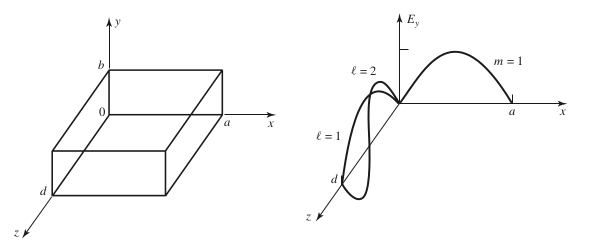
\includegraphics[scale=0.5]{rectres}
  \caption{Ressonador paral·lelepipèdic i els seus camps ressonants }
  \label{rectres}
\end{figure}

\begin{equation}
  \nonumber
  \begin{array}{ccc}
    e_z^+  = E_0 ^+ \bar{e_z ^+} & e_x^+ = E_0 ^+ \bar {e_x ^+} & e_y ^+ = E_0 ^+ \bar{e_y ^+} \\
    h_z ^+ = 0 & h_x ^+ = E_0 ^+ \bar {h_x ^+} & h_y^ + = E_0 ^+ \bar {h_x ^+} \\ 
  \end{array}
\end{equation}

Els camps de la ona $-$ só iguals però canviant $\beta \to -\beta$ i $H_0 ^+ \to H_0 ^-$. En termes dels coeficients  $\bar{e_i ^+}$ queden:
 
\begin{equation}
  \nonumber
  \begin{array}{ccc}
    e_z ^- =  E_0 ^- \bar{e_z ^+} & e_x ^- = -E_0 ^- \bar {e_x ^+} & e_y ^- = -E_0 ^- \bar{e_y ^+} \\
    h_z ^- =  0 & h_x ^- =  E_0 ^- \bar {h_x ^+} & h_y ^- =  E_0 ^- \bar {h_x ^+} \\
  \end{array}
\end{equation}

per a la $-$. Sumant aquestes expressions obtenim les interferències:
\begin{subequations}
  \begin{align}
    E_z &= E_0 ^+ \bar{ e_z ^+} \e{-\jmath \beta z} + E_0 ^- \bar{ e_z ^+} \e{\jmath \beta z} \\
    E_x &= E_0 ^+ \bar{ e_x ^+} \e{-\jmath \beta z} - E_0 ^- \bar{ e_x ^+} \e{\jmath \beta z}  \\
    E_y &= E_0 ^+ \bar{ e_y ^+} \e{-\jmath \beta z} - E_0 ^- \bar{ e_y ^+} \e{\jmath \beta z}  \\    
    H_z &= 0 \\
    H_x &= E_0 ^+ \bar{ h_x ^+} \e{-\jmath \beta z} + E_0 ^- \bar{ h_x ^+} \e{\jmath \beta z}  \\
    H_y &= E_0 ^+ \bar{ h_y ^+} \e{-\jmath \beta z} + E_0 ^- \bar{ h_y ^+} \e{\jmath \beta z} 
  \end{align}
\end{subequations}

Apliquem les condicions de contorn:
\begin{enumerate}
  \item{$E_x (z=0) = 0 \to \bar{e_x ^+} ( E_o ^+ \e{-0} - E_o ^- \e{0}) = 0 \to E_0 ^+ = E_0 ^- $}
  \item{$E_x (z=c) = 0 \to \bar{e_x ^ +} E_0 ^+ ( \e{- \jmath \beta c} - \e{\jmath \beta c}) = 0 \to \sin \beta c = 0 \to \beta c = l \pi$ amb $l \in \Zahl$}
\end{enumerate}

Les freqüències d' aquestes ones són les de ressonància:
\begin{equation}
 \beta ^2 =  \omega ^ 2 \mu \epsilon - \left ( \frac{n \pi}{a} \right ) - \left ( \frac{m \pi}{b} \right ) = \left ( \frac{l\pi}{c} \right ) ^2 \to  \omega _{mnl} = \frac{1}{\sqrt{\mu \epsilon}} \sqrt{ \left ( \frac{n \pi}{a} \right ) + \left ( \frac{m \pi}{b} \right ) + \left ( \frac{l \pi}{c} \right )}
\end{equation}

\subsubsection{Cavitat circular}

Per a trobar les freqüències de ressonància d' una guia circular curtcircuitada (figura \cref{circres}) procedim com abans: escrivim els camps dels modes $TE_{mn}$ en direcció $+z$ i $-z$, els sumem i apliquem les condicions de contorn $E_{\varphi}(z=0) = E_s (z=0) = 0$ i $E_{\varphi}(z=c) = E_s (z=c) = 0$, i obtenim la restricció per a $\beta$, que és la mateixa d' abans: $\beta c = l \pi$ amb $l \in \Zahl$. 

\begin{figure}[ht]
  \centering
  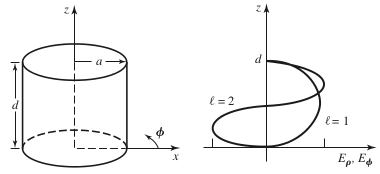
\includegraphics[scale=0.5]{circres}
  \caption{Ressonador paral·lelepipèdic i els seus camps ressonants }
  \label{circres}
\end{figure}

Les freqüències de ressonància són per tant 

\begin{equation}
  \beta ^2 = \omega ^2 \mu \epsilon - \left ( \frac{P_{mn}}{a} \right ) ^2 = \left ( \frac{l\pi}{c} \right ) \to \omega _{mnl} = \sqrt{\left ( \frac{P_{nm}}{a} \right ) ^2 + \left ( \frac{n}{c} \right ) ^2 }
\end{equation}


\chapter{Mètodes pertorbatius i modes acoblats}

\section{Introducció}

Encara que podem resoldre problemes molt complexos mitjançant càlcul numèric, ens interessa obtindre solucions analítiques, encara que siguen aproximades, per a alguns casos. Als ressonadors, per exemple, podem calcular les freqüències de ressonància, però si fem un forat per introduir els camps canviem les condicions de contorn i, molt probablement, deixem de tindre solució analítica. Igualment, quan dues línies dielèctriques s' apropen massa els modes s' acoblen i deixem de tindre solucions. Aquests són dos exemples de situacions que, com vorem, podem resoldre usant mètodes pertorbatius i teoria de modes acoblats, respectivament.

\section{Mètodes pertorbatius}

Els mètodes pertorbatius ens permeten calcular, a partir dels camps electromagnètics d' un sistema, els camps d' un sistema idèntic al primer excepte per xicotetes diferències anomenades pertorbacions. Hi ha dos tipus principals de pertorbacions: pertorbacions de forma i pertorbacions del material.

\subsection{Pertorbacions materials}

Tenim un sistema ressonant del que coneixem les $\omega _0$, i volem trobar les noves $\omega _0$ en cas de que fem un xicotet canvi $\epsilon \to \epsilon + \Delta \epsilon$ i $\mu \to \mu + \Delta \mu$ a les propietats del material (figura \cref{perturbmaterial}). Els camps originals satisfan:

\begin{figure}[ht]
  \centering
  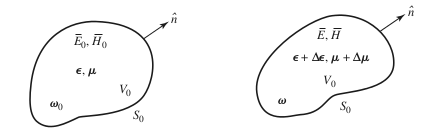
\includegraphics[scale=0.5]{perturbmaterial}
  \caption{Sistema original i sistema amb propietats pertorbades}
  \label{perturbmaterial}
\end{figure}

\begin{subequations}
  \begin{align}
    \del \times \vec E_0 &= - \jmath  \omega _0 \mu \vec H_0 \label{ori1}\\
    \del \times \vec H_0 &=  \jmath  \omega _0 \epsilon \vec E_0 \label{ori2} 
  \end{align}
\end{subequations}

I els del sistema pertorbat satisfan

\begin{subequations}
  \begin{align}
    \del \times \vec E &= - \jmath  \omega (\mu + \Delta \mu) \vec H \label{new1} \\
    \del \times \vec E &= \jmath  \omega (\epsilon + \Delta \epsilon) \vec H \label{new2}
  \end{align}
\end{subequations}

Multipliquem  \cref{ori1}$^*$ per $\vec H$ i restem $\vec E^* \cdot$ \cref{new2}

\begin{equation}
  \del (\vec E_0^* \times \vec H_0 ) = \jmath \omega_0 \mu \vec H_0^* \cdot \vec H - \jmath \omega (\epsilon + \Delta \epsilon) \vec E_0 ^* \cdot \vec E \label{eq5}
 \end{equation}

I fent $\vec E \cdot$ \cref{ori2}$^*$ - $\vec H_0 ^*$ \cref{new1}

\begin{equation}
  \del (\vec E_0 \times \vec H_0 ^*) = \jmath \omega \epsilon \vec E_0^* \cdot \vec E - \jmath \omega (\mu + \Delta \mu) \vec H_0 ^* \cdot \vec H \label{eq6}
\end{equation}

Integrem la suma de \cref{eq5,eq6}:

\begin{equation}
  \begin{aligned}
  \int _{V_0} \del ( \vec E_0 ^* \times \vec H + \vec E \times \vec H_0 ^*) dV = \int \bigg [ &\jmath ( \omega_0 - \omega) \epsilon \vec E_0 ^* \cdot \vec E + \jmath (\omega_0 - \omega) \mu \vec H_0 ^* \cdot \vec H \\
  - &\jmath \omega \Delta \epsilon \vec E _0 ^* \cdot \vec E - \jmath \omega \Delta \mu \vec H_0 ^ * \cdot \vec H \bigg ] dV
  \end{aligned}  
\end{equation}

Usem el teorema de la divergència en la primera integral

\begin{equation}
  \begin{aligned}
  \int _{S_0}  (\vec E_0 ^* \times \vec H + \vec E \times \vec H_0 ^*) \cdot \vec dS = \int \bigg [ &\jmath ( \omega_0 - \omega) \epsilon \vec E_0 ^* \cdot \vec E + \jmath (\omega_0 - \omega) \mu \vec H_0 ^* \cdot \vec H \\
  - &\jmath \omega \Delta \epsilon \vec E _0 ^* \cdot \vec E - \jmath \omega \Delta \mu \vec H_0 ^ * \cdot \vec H \bigg ] dV \label{integral}
  \end{aligned}
\end{equation}

Com que els camps elèctrics són perpendiculars a la superfície la integral sobre $S$ és zero, i manipulant els termes de la integral sobre $V$ obtenim

\begin{equation}
  \frac{\omega - \omega _0}{\omega} = \frac{\int _{V_0} \left [ \Delta \epsilon \vec E_0 ^* \cdot \vec E + \Delta \mu \vec H_0 ^* \cdot \vec H \right ] dV}{\int _{V_0} \left [ \epsilon \vec E _0 ^ * \cdot \vec E + \mu \vec H_0 ^* \cdot \vec H \right] dV}
\end{equation}

Si coneguérem $\vec E_0$, $\vec H_0$, $\vec E$ i $\vec H$ podríem calcular $\omega$ exactament. Com que no els coneguem assumirem  que $\vec E \simeq \vec E_0$ i $\vec H \simeq \vec H_0$, ja que $\Delta \epsilon$ i $\Delta \mu$ són molt xicotets.

\begin{equation}
  \frac{\omega - \omega _0}{\omega} = \frac{\int _{V_0} \left [ \Delta \epsilon \vec E_0 ^* \cdot \vec E_0 + \Delta \mu \vec H_0 ^* \cdot \vec H_0 \right ] dV}{\int _{V} \left [ \epsilon \vec E_0 ^ * \cdot \vec E_0 + \mu \vec H_0 ^* \cdot \vec H_0 \right] dV} = \frac{\Delta W}{W}
\end{equation}

La última igualtat, on $W$ és la energia emmagatzemada als camps, es deu a que les integrals són les del teorema de Poynting. Noteu que cal integrar el denominador sobre tot el volum $V_0$, però el numerador pot acotar-se a la zona pertorbada.

\subsection{Pertorbació de forma}

Si la pertorbació consisteix en un canvi en la forma, i no en els materials (figura \cref{perturbshape}), repetim el procés anterior fins a arribar a \cref{integral}, amb la diferència de que ara $\Delta \epsilon = \Delta \mu = 0$:

\begin{figure}[ht]
  \centering
  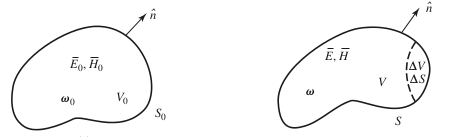
\includegraphics[scale=0.5]{perturbshape}
  \caption{Sistema original i sistema amb forma pertorbada}
  \label{perturbshape}
\end{figure}

\begin{equation}
  \int _{S_0}  (\vec E_0 ^* \times \vec H + \vec E \times \vec H_0 ^*) \cdot \vec dS = \jmath ( \omega_0 - \omega) \int \left [  \epsilon \vec E_0 ^* \cdot \vec E + \mu \vec H_0 ^* \cdot \vec H \right ] dV
\end{equation}

i podem arribar a l' expressió exacta 
\begin{equation}
  \omega - \omega_0 = \frac{- \jmath \oint _{\Delta S} \vec E_0 ^* \times \vec H_0 \vec dS}{\int _V (\epsilon \vec E_0 \cdot \vec E_0 ^* + \mu \vec H_0 \cdot \vec H_0^*) dV}
\end{equation}

On hem suposat, com abans, que $\vec E \simeq \vec E_0$ i $\vec H \simeq \vec H_0$, ja que $\Delta S \simeq 0$. També com abans podem integrar el numerador solament en la zona pertorbada.

\section{Teoria de modes acoblats}

De vegades passa que dos modes interaccionen entre ells de manera que hi ha un transvasament d' energia d' un a l' altre, com en els acobladors de senyal, en estructures periòdiques en moduladors acusto-òptics, en amplificadors... La teoria de modes acoblats ens permet obtindre el resultat d' acoblaments com aquests, i és més general: pot ser aplicada a modes no electromagnètiques, o a acoblaments entre modes EM i no EM (com acústics, o ones d' electrons).

\subsection{Acoblament de modes copropagants}

Si en una guia en la que es propaga més d' un mode de manera independent fem una pertorbació podem provocar que els modes deixen de ser independents. Suposem que el mode resultant és una combinació lineal dels modes originals 1 i 2:

\begin{subequations}
  \begin{align}
    \vec E ' &= A_1(z) \vec E_1 e^{-\jmath \beta_1 z} + A_2 (z) \vec E_2 e^{-\jmath \beta _2 z } \\
    \vec H ' &= A_1 (z) \vec H_1 e^{-\jmath \beta _1 z} + A_2 (z) \vec H_2 e^{-\jmath \beta_2 z}
  \end{align}
\end{subequations}

i intentem trobar $A_1(z)$ i $A_2(z)$. Per un procediment similar al de la secció anterior arribem a la igualtat

\begin{equation}
  \del \left [ A_1(z) (\vec E_1^* \times \vec H_1 + \vec E_1 \times \vec H_1 ^ * ) + A_2 (z) (\vec E_1 ^* \times \vec H_2 +  \vec E_2 \times \vec H_1 ^* ) \right ] = - \jmath \omega \Delta \epsilon  \vec E_1 ^* \cdot \vec E \label{igualtat}
\end{equation}

Integrem ambdós costats sobre la secció transversal $S_t$ i apliquem el teorema de la divergència en 2 dimensions. Anomenant $\vec F$ a la suma dins del $\del$ en \cref{igualtat} arribem a

\begin{equation}
  \pd{}{z} \int_{S_t} \vec F \cdot \vec dS + \oint _{C(S_t)} \vec F \cdot \vec n dl = - \jmath \omega \Delta \epsilon \int _{S_t} \vec E_1 ^* \cdot \vec E dS
\end{equation}

En cas de que les parets siguen conductores la integral de contorn desapareixerà, ja que $\vec E \times \vec H$ és tangent a aquestes. Si són dielèctriques el integrant és proporcional a $\frac{1}{r}$, i considerant contorns infinits deduïm que ha d' anul·lar-se igualment.

Si reescrivim $\vec F$ explícitament i calculem la derivada sobre la integral arribem a:

\begin{equation}
  \begin{aligned}
  \pd{A_1}{z} &= -\jmath \omega \int \left[ \Delta \epsilon \vec E_1 ^* e^{-\jmath \beta _1 z} ( A_1 e^{\jmath \beta _1 z} \vec E_1 + A_2 e^{\jmath \beta _2 z} \vec E_2) \right] dS \\
  &= k_{11} A_1 (z) + k_{12} A_2(z) e^{\jmath \delta z}
  \end{aligned}
\end{equation}

On hem definit 

\begin{subequations}
  \begin{align}
    \delta &= \beta_2 - \beta_1 \nonumber \\
    k_{11} &= -\jmath \omega \int \Delta \epsilon \abs{\vec E_1} ^2 dS \nonumber \\
    k_{12}& = -\jmath \omega \int \Delta \epsilon \vec E_1 ^* \cdot \vec E_2 dS \nonumber \\
  \end{align}
\end{subequations}

I, similarment,

\begin{equation}
  \pd{A_2}{z} = k_{22} A_2 (z) + k_{21} A_1(z) e^{\jmath \delta z}
\end{equation}

amb

\begin{subequations}
  \begin{align}
    k_{22} &= -\jmath \omega \int \Delta \epsilon \abs{\vec E_2} ^2 dS \nonumber \\
    k_{12} &= k_{21}^* \nonumber \\
  \end{align}
\end{subequations}

D' aquestes dues equacions podem calcular $A_1$, i $A_2$ en funció de $\delta$ i $\epsilon$. En general observarem que les seues amplituds $\abs{A_1}^2$ i $\abs{A_2} ^2$ estan en contrafase, ja que l' energia que un dels modes perd el guanya l' altre.

\chapter{Teoria de circuits d' alta freqüència}

\section{Introducció}

Un dispositiu en un circuit d' alta freqüència es representa com una caixa negra amb diversos ports (o canals) d' entrada i eixida. Cada un d' aquests ports és una guia d' ones representada com a dos terminals als que existeix una tensió i una corrent d' entrada i eixida. Ens interessa trobar les funcions de transferència d' aquests dispositius (les relacions entre cada entrada i cada eixida). Aquestes funcions poden calcular-se per dues vies diferents: teoria de circuits (trobant la matriu d' impedàncies o d' admitàncies) o per teoria d' ones (trobant la matriu de dispersió o scattering).

\section{V i I en una guia d' ona}

Intentem obtindre el V i I d' una guia d' ones a partir dels seus camps $\rfield{E}$ i $\rfield{H}$.  Denotem els camps d' entrada i eixida amb + i - i definim $\vp$ i $\ip$:
\begin{align}
  \rfield{E}_t ^+ = E_0 ^+ \vec e_t (x, y) e^{j(\omega t - \beta z)} = \frac{\vp}{c_1} \vec e_t(x, y) e^{j(\omega t - \beta z)} \\
  \rfield{H}_t ^+ = E_0 ^+ \vec e_t (x, y) e^{j(\omega t - \beta z)} = \frac{\ip}{c_2} \vec h_t(x, y) e^{j(\omega t - \beta z)} 
\end{align}

Ara hem de trobar $c_1$ i $c_2$. Comencem igualant les expressions de la potència de la guia segons la teoria d' ones i segons la teoria de circuits.

\begin{align}
  P_{ones} &= \frac{1}{2} \int  ( \rfield{E} \times \rfield{H} ^* ) \uz dS = \frac{1}{2} \frac{\vp \ip}{c_1 c_2 ^*} \int ( \vec e_t \times \vec h_t ) \uz dS  \\
  P_{circuits} &= \frac{1}{2} \vp \ip 
\end{align}

Si han de ser iguals ha de complir-se que
\begin{equation}
  c_1 c_2 ^* = \int ( \vec e_t \times \vec h_t ) \uz dS
\end{equation}

el que ens dona una primera relació entre $c_1$ i $c_2$. La segona relació no sempre existeix. Si el mode és TE, TM o TEM les amplituds dels càlculs estan relacionats per l' admitància o l' impedància: $E_0 ^+ = H_0 ^+ Z$, d' on obtenim
\begin{equation}
  \frac{\vp}{\ip} \frac{c_2}{c_1} = z
\end{equation}

Si el mode és TEM aleshores $\frac{\vp}{\ip} = z_c$ i $z = z_c \frac{c_2}{c_1}$. El mateix anàlisi pot usar-se per a calcular $\vm$ i $\im$.

\section{Matrius d' impedància Z i d' admitància Y}

Suposem un dispositiu amb n entrades, indexades per $j$. En la porta $j$ tindrem
\begin{align}
  V_j &= \vp  + \vm \\
  I_j &= \ip + \im
\end{align}

Si posem una corrent en una o varies portes apareixerà una tensió an algunes de les altres. Definim la matriu d' impedància $Z_{ij}$ tal que
\begin{equation}
  V_i = \sum_{i = 0} ^N Z_{ij} V_j
\end{equation}

La matriu d' admitàncies es defineix anàlogament
\begin{equation}
  Y_j = \sum _{j=1}^N Y_{ij} Y_j
\end{equation}
%
Quina informació ens proporcionen els elements d' aquestes matrius? Ens donen la relació entre tensió a la porta $i$ i corrent a la porta $j$ quan totes les altres estan en circuit obert:
\begin{align}
  Z_{ij} = \left . \frac{V_i}{I_j} \right \vert \sub{$I_k = 0$ per a $k \neq j$}
\end{align}
o entre corrent a la porta $i$ i tensió a la porta $j$ quan totes les altres estan curtcircuitades:
\begin{equation}
  Y_{ij} = \left . \frac{I_i}{V_j} \right \vert \sub{$V_k = 0$ per a $k \neq j$}
\end{equation}

\section{Matriu d' scattering S}

Alternativament podem definir els paràmetres de potència incident i reflectida:
\begin{equation}
  a_i = \frac{\vp}{\sqrt{Z_{Ci}}} \qquad b_i = \frac{\vm}{\sqrt{Z_{Ci}}}
\end{equation}
anomenats així perquè, a partir de la seua definició, podem arribar a la igualtat
\begin{equation}
  P_i = \frac{1}{2} \Re \left [ \left \vert a_i \right \vert ^2 - \left \vert b_i \right \vert ^2 \right ]
\end{equation}

que podem interpretar com a la potència entrant al port $i$ menys la potència eixint del port $i$. A partir d' aquests coeficients podem definir els  paràmetres S:
\begin{equation}
  S_{ij} = \left . \frac{b_i}{a_j} \right \vert \sub{$a_k = 0$ per a $k \neq j$}
\end{equation}

tals que
  
\begin{equation}
  b_i = \sum_j S_{ij} a_j
\end{equation}

La informació continguda en aquest paràmetres és els paràmetres de reflexió (quan $i = j$) i els de transmissió (quan $i \neq j$):
\begin{align}
  S_{ii} = \frac{V_i ^-}{V_i^+} \\
  S_{ij} =  \sqrt{\frac{Z_{Cj}}{Z_{Ci}}}  \frac{V_i ^-}{V_j ^+}
\end{align}

Podem mesurar els paràmetres $S$ d' una xarxa amb dues portes usant un analitzador de xarxes vectorial (VNA). Per a dispositius més complixats d'$n$ portes utilitzem el VNA i analitzem les portes per parells. Noteu que, segons la definició, quan mesurem el paràmetre $S_{ij}$ haurem d' assegurar-nos de que totes les portes que no siguen $j$ estiguen adaptades, per a que no hi haja reflexions.

\section{Propietats de les matrius}

En sistemes recíprocs (passius, no aporten energia) $Z$ i $Y$ son simétriques. Si no hi ha pèrdues són, a més, imaginàries pures.

Depenent del problema una matriu serà més ñutil que l' altra, pel que és útil saber obtindre'n una de l' altra. De la definició dels paràmetres $a_i$ i $b_i$ obtenim
\begin{align}
  a_i + b_i &= \frac{V_i ^+ + V_i ^-}{\sqrt{Z_{ci}}} = \frac{V_i}{\sqrt{Z_{ci}}} \\
  a_i - b_i &= \frac{V_i ^+ - V_i ^-}{\sqrt{Z_{ci}}} = \sqrt{Z_{ci}} I_i
\end{align}

Sumant i restant aquestes dos equacions:
\begin{align}
  a_i = \frac{1}{2} \left ( \frac{V_i}{\sqrt{Z_{ci}}} + \sqrt{Z_{ci}} I_i \right ) = \frac{1}{2} \left ( \frac{1}{\sqrt{Z_{ci}}} \sum_j Z_{ij} I_j + \sqrt{Z_{ii}} I_i \right )  \\
  b_i = \frac{1}{2} \left ( \frac{V_i}{\sqrt{Z_{ci}}} - \sqrt{Z_{ci}} I_i \right ) = \frac{1}{2} \left ( \frac{1}{\sqrt{Z_{ci}}} \sum_j Z_{ij} I_j + \sqrt{Z_{ii}} I_i \right  )
\end{align}

Definint les matrius
\begin{align}
  Z_{ij} ^{D+} = \frac{Z_{ij}}{\sqrt{Z_{ci}}} + \delta _{ij} \sqrt{Z_{ci}} \\
  Z_{ij} ^{D-} = \frac{Z_{ij}}{\sqrt{Z_{ci}}} - \delta _{ij} \sqrt{Z_{ci}}
\end{align}
podem expressar els coeficients com a
\begin{align}
  a_i = \sum_j Z_{ij}^{D+} I_j \\
  b_i = \sum_j Z_{ij}^{D-} I_j
\end{align}
o, en termes dels vectors que contenen els coeficients i les corrents de cada porta $\vec a = Z^{D+} \vec I$ i $\vec b = Z^{D-} \vec I$.
Ara podem, de la definició de $S$
\begin{equation}
  \vec b = S \vec a
\end{equation}

obtindre la relació d' aquesta amb $Z$:
\begin{equation}
  S = Z^{D-} \left [ Z^{D+} \right ] ^{-1}
\end{equation}

Les propietats de $Z$ es translladen a $S$: en sistemes recíprocs $S$ és simètrica, i per tant ens podem estalviar la meitat de les mesures. Noteu que per a un sistema biporta
\begin{align}
  \abs {S_{11}} ^2 +  \abs {S_{22}} ^2 = 1 \\
  \abs {S_{21}} ^2 +  \abs {S_{12}} ^2 = 1 
\end{align}

\section{Conexions de xarxes en cascada}

Els elements de les matrius d' scattering i d' impedància tenen significat físic i són per tant directament mesurables, però tenen l' inconvenient de que no són multiplicatives. És a dir, la matriu $S$ d' una xaxa composada per dos xarxes amb matrius $S_1$ i $S_2$ no és $S_1 S_2$. És per això que definim la matriu T
\begin{equation}
  \left [ \begin{array}{c} b_2 \\ a_2 \end{array}  \right ] = T \left [ \begin{array}{c} a_1 \\ b_1 \end{array} \right ]
\end{equation}
que si que satisfá aquesta propietat. Les expressions per a passar de la matriu S a la T i viceversa són
\begin{equation}
  T = \left [
    \begin{array}{cc}
      \frac{\operatorname{det}(S)}{S_{12}} & \frac{S_{22}}{S_{12}} \\ [1.5ex] 
      - \frac{S_{11}}{S_{12}} & \frac{1}{S_{12}}
    \end{array}
    \right ]
    \qquad
    S = \left [
    \begin{array}{cc}
      - \frac{T_{21}}{T_{22}} & \frac{1}{T_{22}} \\ [1.5ex] 
        \frac{\operatorname{det}(T)}{T_{22}} & \frac{T_{12}}{T_{22}}
    \end{array}
    \right ]
\end{equation}



%\appendix 

%\chapter{Funcions de Bessel}

Les funcions de Bessel bla bla bla

\end{document}

%%% Local Variables:
%%% mode: latex
%%% TeX-master: t
%%% End:
